\documentclass[a4paper,oneside,12pt]{book}
\usepackage{geometry}
\geometry{top=15mm, left=10mm, right=10mm, bottom=15mm}
\usepackage{amsmath}  % สำคัญมาก: ช่วยให้ใช้งานคำสั่ง \text{} ในสูตรคณิตศาสตร์ได้
\usepackage{amssymb}  % ช่วยเพิ่มสัญลักษณ์คณิตศาสตร์อื่นๆ
\usepackage{fontspec}
\usepackage{xltxtra}
%\usepackage{polyglossia}
\usepackage{tcolorbox}
\tcbuselibrary{skins, breakable}
\usepackage{tikz}
\usepackage{titlesec}
\usepackage{xcolor}

% ----------  \begin{enumerate}[label*=\arabic*.]----------
\usepackage{enumitem}


\usepackage{varwidth} % <--- 🌟 พระเอกของงานนี้ ต้องใส่ตัวนี้นะครับ
\usepackage{ragged2e}

% ----------แทรกรูปให้ล๊อคตำแหน่ง ----------
\usepackage{caption}
%\captionsetup[figure]{name=Figure}
\usepackage{graphicx} % สำหรับแทรกรูป
\usepackage{float}    % <-- อันนี้สำคัญ



\usepackage{array}
\usepackage{multicol}
\usepackage{cellspace} % ช่วยเพิ่มช่องว่างบน-ล่างให้เซลล์อัตโนมัติ
\setlength\cellspacetoplimit{6pt}
\setlength\cellspacebottomlimit{6pt}


\renewcommand{\chaptername}{บทที่}
\renewcommand{\contentsname}{สารบัญ}
\renewcommand{\figurename}{รูปที่}

% ตั้งค่าฟอนต์ Mathematics
%\usepackage{unicode-math}
%\usepackage{gfsneohellenicot}

\usepackage{unicode-math} 
\setmainfont{GFS Neohellenic}[Scale=1.3]
\setmathfont{GFS Neohellenic Math}[Scale=1.3]
% ตั้งค่าฟอนต์หลักเป็น GFS Neohellenic สำหรับภาษาอังกฤษ
%\setmainfont{GFS Neohellenic}

%\DeclareMathSizes{12}{14}{10}{7} % ใช้ปรับขนาดฟอนต์ Math
%\usepackage{concmath}
%\usepackage[OT1]{fontenc}


%\usepackage{pxfonts}
%\usepackage[T1]{fontenc}

% ---- math operators ----
\DeclareMathOperator{\arcsec}{arcsec}
\DeclareMathOperator{\arccosec}{arccosec}
\DeclareMathOperator{\arccot}{arccot}
\DeclareMathOperator{\cosec}{cosec}



%\setdefaultlanguage{thai}
%\setotherlanguage{english}

% ตั้งค่าฟอนต์
\setmainfont[
Extension = .ttf,
UprightFont = THSarabunNew,
BoldFont = THSarabunNew Bold,
ItalicFont = THSarabunNew Italic,
BoldItalicFont = THSarabunNew BoldItalic,
Scale = 1.5
]{THSarabunNew}

\newfontfamily\thaifont[
Extension = .ttf,
UprightFont = THSarabunNew,
BoldFont = THSarabunNew Bold,
ItalicFont = THSarabunNew Italic,
BoldItalicFont = THSarabunNew BoldItalic,
Scale = 1.5
]{THSarabunNew}

\XeTeXlinebreaklocale "th"
\XeTeXlinebreakskip = 0pt plus 1pt

\makeatletter
% [ส่วนที่ 1] สไตล์ CHAPTER
\newcommand{\drawchapterbox}[1]{%
	\begin{tcolorbox}[
		enhanced,                      % จำเป็นสำหรับการใช้ shadow
		colback=white, 
		colframe=black, 
		sharp corners, 
		boxrule=1.5pt, 
		halign=flush center, 
		top=22pt, bottom=22pt, left=15pt, right=15pt, 
		before skip=0pt, after skip=0pt,
		% --- เพิ่มส่วนของเงา ---
		shadow={2mm}{-2mm}{0mm}{black!30}, 
		% หมายเหตุ: {2mm} คือเลื่อนขวา, {-2mm} คือเลื่อนลง, {0mm} คือความฟุ้ง, {black!30} คือสีเงา
		]
		\centering
		\ifnum\value{chapter}>0
		{\huge\bfseries\chaptername~\thechapter}\par\vspace{15pt} 
		\fi
		{\Huge\bfseries #1}
	\end{tcolorbox}
}
\titleformat{\chapter}[block]{\normalfont}{}{0pt}{\drawchapterbox}
\titlespacing*{\chapter}{0pt}{0pt}{8pt}
\assignpagestyle{\chapter}{empty}

% ==================================================
% [ส่วนที่ 2] สีและสไตล์กล่องสำหรับ SECTION / SUBSECTION
% ==================================================
\usepackage{xcolor}
\usepackage{tcolorbox}
\tcbuselibrary{skins, breakable}

% นิยามเฉดสีธีม Deep Navy & Slate สไตล์อินเตอร์เนชันแนล
\definecolor{TopNavy}{RGB}{31, 58, 98}
\definecolor{SubSlate}{RGB}{90, 105, 120}

% 1. แถบหัวข้อหลัก (Section): แถบริบบิ้นทึบพาดเต็มหน้าลอยละมุน
\newtcolorbox{sectionfullbox}[1][]{
	enhanced, breakable,
	colback=TopNavy,                
	colframe=TopNavy,
	boxrule=0pt, sharp corners,
	left=15pt, right=15pt, top=8pt, bottom=8pt,
	fontupper=\Large\bfseries\color{white}, 
	fuzzy shadow={0mm}{-1mm}{0mm}{1mm}{black!15}, 
	before upper={\RaggedRight\hspace{0pt}},
	#1
}

% 2. แถบหัวข้อย่อย (Subsection): เปิดขอบซ้ายหนา 4pt ด้านอื่นโล่ง สยบปัญหาคำตก
\newtcolorbox{subsectiontitlebox}[1][]{
	enhanced, breakable,
	colback=SubSlate!6!white,       
	colframe=SubSlate,
	boxrule=0pt, leftrule=4pt,      
	sharp corners,
	left=12pt, right=15pt, top=6pt, bottom=6pt, 
	fontupper=\large\bfseries\color{SubSlate!90!black},
	before upper={\RaggedRight\hspace{0pt}},
	#1
}

% ==================================================
% [ส่วนที่ 3] โครงสร้างระบบลอจิกอัตโนมัติ (เวอร์ชันขยับระยะกระชับเนี๊ยบ)
% ==================================================
\makeatletter

% --- ตั้งค่าระยะ Padding ของกล่องนอก ---
\newlength\SectionPad
\setlength{\SectionPad}{24pt}
\newlength\SubsectionPad
\setlength{\SubsectionPad}{20pt}

% --- SECTION SYSTEM ---
\renewcommand{\section}{\@ifstar{\sectionstar}{\sectionnormal}}

\newcommand{\sectionnormal}[1]{%
	\refstepcounter{section}%
	\addcontentsline{toc}{section}{\protect\numberline{\thesection}#1}%
	\markright{\thesection\ #1}%
	\begingroup
	\vspace{12pt}%      % ปรับลดระยะเหนือกหัวข้อใหญ่เล็กน้อยเพื่อความสมดุล
	\begin{sectionfullbox}[hbox, before upper={\RaggedRight}]
		\begin{varwidth}{\dimexpr\linewidth-\SectionPad\relax}
			\noindent
			\Large\bfseries \thesection\hspace{0.5em}#1
		\end{varwidth}
	\end{sectionfullbox}
	\par\endgroup
	\vspace{4pt}%       % 🛠️ จุดสำคัญ: ลดระยะท้าย Section ลงเหลือ 4pt (จากเดิม 10pt) เพื่อดึงขอบล่างขยับชิดขึ้น
	\@afterheading%
}

\newcommand{\sectionstar}[1]{%
	\begingroup
	\vspace{12pt}%
	\begin{sectionfullbox}[hbox, before upper={\RaggedRight}]
		\begin{varwidth}{\dimexpr\linewidth-\SectionPad\relax}
			\noindent
			\Large\bfseries #1
		\end{varwidth}
	\end{sectionfullbox}
	\par\endgroup
	\vspace{4pt}%       % 🛠️ ลดระยะท้ายลงเหลือ 4pt เช่นกัน
	\@afterheading
}

% --- SUBSECTION SYSTEM ---
\renewcommand{\subsection}{\@ifstar{\subsectionstar}{\subsectionnormal}}

\newcommand{\subsectionnormal}[1]{%
	\refstepcounter{subsection}%
	\addcontentsline{toc}{subsection}{\protect\numberline{\thesubsection}#1}%
	\begingroup
	% 🛠️ จุดสำคัญ: แก้ไขลอจิกเช็คระยะห่าง ถ้าเกิดตามหลัง \section ทันที ให้ลดแรงดีดแนวตั้งเหลือแค่ 2pt 
	\ifnum\value{subsection}=1
	\vspace{2pt}%
	\else
	\vspace{8pt}%   % ถ้าเป็นหัวข้อย่อยถัด ๆ ไปในเนื้อหาปกติ ให้เว้นระยะห่างตามมาตรฐานพอดี ๆ
	\fi
	\begin{subsectiontitlebox}[hbox, before upper={\RaggedRight}]
		\begin{varwidth}{\dimexpr\linewidth-\SubsectionPad\relax}
			\noindent
			\large\bfseries \thesubsection\hspace{0.5em}#1
		\end{varwidth}
	\end{subsectiontitlebox}
	\par\endgroup
	\vspace{6pt}%       % ปรับระยะก่อนเริ่มเนื้อหาบทเรียนให้กระชับพอดีสายตา
	\@afterheading
}

\newcommand{\subsectionstar}[1]{%
	\begingroup
	\vspace{6pt}%
	\begin{subsectiontitlebox}[hbox, before upper={\RaggedRight}]
		\begin{varwidth}{\dimexpr\linewidth-\SubsectionPad\relax}
			\noindent
			\large\bfseries #1
		\end{varwidth}
	\end{subsectiontitlebox}
	\par\endgroup
	\vspace{6pt}%
	\@afterheading
}

\makeatother
% ==========================================
% 4. ระบบกล่องข้อความคณิตศาสตร์ (tcolorbox)
% ==========================================
\definecolor{brilliantlavender}{rgb}{0.75, 0.58, 0.89}
\definecolor{darkseagreen}{rgb}{0.56, 0.74, 0.56}
\definecolor{magentaprocess}{rgb}{1.0, 0.0, 0.56} 
\definecolor{asparagus}{rgb}{0.53, 0.66, 0.42}

\newcounter{definition}[chapter]
\renewcommand{\thedefinition}{\thechapter.\arabic{definition}}

\newcounter{theorem}[chapter]
\renewcommand{\thetheorem}{\thechapter.\arabic{theorem}}

\newcounter{example}[chapter]
\renewcommand{\theexample}{\thechapter.\arabic{example}}

\newcounter{remark}[chapter]
\renewcommand{\theremark}{\thechapter.\arabic{remark}}

\newcounter{agreement}[chapter]
\renewcommand{\theagreement}{\thechapter.\arabic{agreement}}

\newcounter{observation}[chapter]
\renewcommand{\theobservation}{\thechapter.\arabic{observation}}

\newcounter{concept}[chapter]
\renewcommand{\theconcept}{\thechapter.\arabic{concept}}

% ==========================================
% 5. สภาพแวดล้อมกล่องแบบต่าง ๆ (Environments)
% ==========================================

\newenvironment{definitionbox}[1][]{%
	\refstepcounter{definition}%
	\begin{tcolorbox}[
		enhanced, breakable, before skip=10pt, after skip=10pt,     
		colback=magenta!5!white, colframe=magenta!80!black, fonttitle=\bfseries,
		coltitle=white, colbacktitle=magenta!80!black,
		attach boxed title to top left={yshift=-2mm, xshift=2mm},
		boxed title style={sharp corners, size=small, colframe=magenta!80!black, colback=magenta!80!black},
		sharp corners, boxrule=1.2pt, arc=0mm, shadow={3.5mm}{-2mm}{0mm}{black!20}, 
		title={\textcolor{white}{บทนิยาม~\thedefinition\if\relax\detokenize{#1}\relax\else: #1\fi}},
		]
	}{%
	\end{tcolorbox}
}

% นิยามสีแดงทับทิมเข้ม
\definecolor{TheoremRed}{RGB}{166, 25, 46}

\newenvironment{theorembox}[1][]{%
	\refstepcounter{theorem}%
	\begin{tcolorbox}[
		enhanced, breakable, before skip=10pt, after skip=10pt,     
		colback=TheoremRed!5!white,       % พื้นหลังสีชมพูจางมากๆ สบายตา
		colframe=TheoremRed,              % สีเส้นขอบกล่องหลัก
		fonttitle=\bfseries,
		coltitle=white, 
		colbacktitle=TheoremRed,
		attach boxed title to top left={yshift=-2mm, xshift=3.5mm},
		boxed title style={sharp corners, size=small, colframe=TheoremRed, colback=TheoremRed},
		sharp corners, 
		boxrule=1.2pt, arc=0mm, 
		shadow={3.5mm}{-2mm}{0mm}{black!15}, % ปรับเงาให้นุ่มนวลขึ้นเล็กน้อยด้วย black!15
		title={\textcolor{white}{ทฤษฎีบท~\thetheorem\if\relax\detokenize{#1}\relax\else: #1\fi}},
		]
	}{%
	\end{tcolorbox}
}

\definecolor{ExampleOrange}{RGB}{184, 78, 34}       % สีส้มอิฐพรีเมียม ตัดสีกรมท่าและทองได้เด่นชัดมาก
\definecolor{ExampleOrangeBg}{RGB}{255, 248, 245}   % พื้นหลังสีส้มพาสเทลจาง ๆ สบายตา

\newenvironment{examplebox}[1][]{%
	\refstepcounter{example}%
	\if\relax\detokenize{#1}\relax \def\mytitle{ตัวอย่าง~\theexample}%
	\else \def\mytitle{ตัวอย่าง~\theexample: #1}\fi
	\begin{tcolorbox}[
		enhanced, breakable, before skip=14pt, after skip=14pt,
		colback=ExampleOrangeBg,
		colframe=ExampleOrange,
		fonttitle=\bfseries\small, 
		coltitle=white, 
		colbacktitle=ExampleOrange,   
		attach boxed title to top left={yshift=-2mm, xshift=5mm},
		boxed title style={
			sharp corners, 
			size=small, 
			colframe=ExampleOrange, 
			colback=ExampleOrange,
			boxrule=0pt,
			arc=1mm, % ให้ขอบป้ายมนเล็กน้อยเพื่อเพิ่มมิติด้านดีไซน์
			top=3pt, bottom=3pt, left=8pt, right=8pt
		},
		sharp corners, 
		boxrule=0.5pt, % เส้นกรอบบางลงเพื่อให้ดูคลีนและโปร่งตาขึ้น
		title={\textcolor{white}{\mytitle}},
		fuzzy shadow={0mm}{-0.5mm}{0mm}{0.5mm}{black!6}
		]
	}{%
	\end{tcolorbox}
}

% --- เวอร์ชันความยาวเต็มหน้า (exampleboxfull) ---
\newenvironment{exampleboxfull}[1][]{%
	\refstepcounter{example}%
	\if\relax\detokenize{#1}\relax \def\exampletitle{ตัวอย่าง~\theexample}%
	\else \def\exampletitle{ตัวอย่าง~\theexample: #1}\fi
	\begin{tcolorbox}[
		enhanced, breakable, height fill, before skip=14pt, after skip=14pt,
		colback=ExampleOrangeBg,
		colframe=ExampleOrange,
		fonttitle=\bfseries\small, coltitle=white, colbacktitle=ExampleOrange,
		attach boxed title to top left={yshift=-2mm, xshift=5mm},
		boxed title style={sharp corners, size=small, colframe=ExampleOrange, colback=ExampleOrange, boxrule=0pt, arc=1mm, top=3pt, bottom=3pt, left=8pt, right=8pt},
		sharp corners, boxrule=0.5pt,
		title={\textcolor{white}{\exampletitle}},
		fuzzy shadow={0mm}{-0.5mm}{0mm}{0.5mm}{black!6}
		]
	}{%
	\end{tcolorbox}
}

\newenvironment{remarkbox}[1][]{%
	\refstepcounter{remark}%
	\begin{tcolorbox}[
		enhanced, breakable, before skip=10pt, after skip=10pt,     
		colback=brilliantlavender!10!white, % ปรับพื้นหลังให้อมม่วงพาสเทลลอยละมุนชัดขึ้นเล็กน้อย (!10)
		colframe=brilliantlavender!80!black, % สีหลักของกล่องหัวเรื่อง (ผสมดำเพื่อให้อ่านตัวหนังสือสีขาวง่าย)
		fonttitle=\bfseries, coltitle=white, 
		colbacktitle=brilliantlavender!80!black, 
		attach boxed title to top center={yshift=-2mm}, % ปรับตำแหน่งหัวข้อให้อยู่ตรงกลางพอดี
		boxed title style={sharp corners, size=small, colframe=brilliantlavender!80!black, colback=brilliantlavender!80!black},
		sharp corners, 
		% จุดเปลี่ยนดีไซน์: ลบคำสั่ง frame code เส้นประเดิมออกทั้งหมด และสั่ง boxrule=0pt เพื่อให้กล่องไร้ขอบ
		boxrule=0pt,
		title={\textcolor{white}{ข้อควรรู้~\theremark\if\relax\detokenize{#1}\relax\else: #1\fi}},
		]
	}{%
	\end{tcolorbox}
}

\definecolor{AgreeBurnt}{RGB}{194, 91, 39}

\newenvironment{agreementbox}[1][]{%
	\refstepcounter{agreement}%
	\begin{tcolorbox}[
		enhanced, breakable, before skip=10pt, after skip=10pt,     
		colback=AgreeBurnt!8!white, 
		colframe=AgreeBurnt, 
		fonttitle=\bfseries, coltitle=white, 
		colbacktitle=AgreeBurnt, 
		attach boxed title to top center={yshift=-2mm},
		boxed title style={sharp corners, size=small, colframe=AgreeBurnt, colback=AgreeBurnt},
		sharp corners, 
		% 🛠️ จุดเด่นดีไซน์: ไร้ขอบ (0pt) แต่สาดเงาสีเบจเข้มเยื้องลงไปด้านล่างขวาแทน
		boxrule=0pt,
		shadow={3mm}{-2mm}{0mm}{AgreeBurnt!20!white},
		title={\textcolor{white}{ข้อตกลง~\theagreement\if\relax\detokenize{#1}\relax\else: #1\fi}},
		]
	}{%
	\end{tcolorbox}
}

\definecolor{ObserveBlue}{RGB}{41, 128, 185}
\newenvironment{observationbox}[1][]{%
	\refstepcounter{observation}%
	\begin{tcolorbox}[
		enhanced, breakable, before skip=10pt, after skip=10pt,     
		colback=ObserveBlue!5!white, 
		fonttitle=\bfseries, coltitle=white, 
		colbacktitle=ObserveBlue, 
		attach boxed title to top center={yshift=-1.5mm},
		boxed title style={sharp corners, size=small, colframe=ObserveBlue, colback=ObserveBlue},
		sharp corners, boxrule=0pt, arc=0mm,
		title={\textcolor{white}{ข้อสังเกต~\theobservation\if\relax\detokenize{#1}\relax\else: #1\fi}},
		frame code={
			\draw[dash pattern=on 4pt off 3pt, line width=1.5pt, color=ObserveBlue] 
			(frame.south west) rectangle (frame.north east);
		}
		]
	}{%
	\end{tcolorbox}
}


\definecolor{ConceptGold}{RGB}{201, 138, 34}      % สีทองหรูสำหรับเน้นจุดสำคัญ
\definecolor{ConceptGoldBg}{RGB}{254, 251, 242}
\newenvironment{conceptbox}[1][]{%
	\refstepcounter{concept}%
	\begin{tcolorbox}[
		enhanced, breakable,
		before skip=14pt, after skip=14pt,
		colback=ConceptGoldBg,              % พื้นหลังครีมงาช้างเดิม
		colframe=ConceptGold,               % เส้นหลักสีทอง
		sharp corners,
		% 🛠️ Layout: เปิดเฉพาะเส้นขอบซ้ายหนา 4pt ด้านอื่นปล่อยโล่งไร้เส้นขอบ
		boxrule=0pt, leftrule=4pt,
		left=12pt, right=12pt, top=10pt, bottom=10pt,
		% 🛠️ ใช้คำสั่ง overlay เพื่อสร้างป้ายหัวเรื่องแบบโมเดิร์นชิดขอบซ้ายในกล่อง
		title={หลักการ~\theconcept\if\relax\detokenize{#1}\relax\else: #1\fi},
		attach title to upper,
		fonttitle=\bfseries\color{ConceptGold}, % สีตัวอักษรหัวเรื่องเป็นสีทองเด่น
		after title={\par\medskip\noindent},    % สั่งขึ้นบรรทัดใหม่เว้นระยะหลังจากป้ายชื่ออย่างสวยงาม
		fuzzy shadow={0mm}{-0.5mm}{0mm}{0.5mm}{black!6}
		]
	}{%
	\end{tcolorbox}
}


\newtcolorbox{mysolution}{
	enhanced,
	colback=white,             % สีพื้นหลังในกล่อง
	colframe=black,            % สีขอบกล่อง
	boxrule=0.8pt,             % ความหนาของเส้นขอบ
	sharp corners,             % มุมฉาก (ถ้าต้องการมุมมนให้แก้เป็น arc=2mm)
	shadow={1.5mm}{-1.5mm}{0mm}{black!30}, % เงาสีดำ
	before skip=10pt, 
	after skip=10pt,
	left=10pt, right=10pt, top=10pt, bottom=10pt,
	title={\bfseries วิธีทำ},
	coltitle=black,            % สีตัวอักษร "วิธีทำ"
	attach boxed title to top left={yshift=-2mm, xshift=2mm},
	boxed title style={
		colback=white,         % พื้นหลังของป้าย "วิธีทำ"
		colframe=white,        % ซ่อนขอบป้ายเพื่อให้กลืนไปกับกรอบ
		sharp corners
	}
}

\makeatother

% เปลี่ยนชื่อเป็น \mysol
% วางไว้ใน Preamble ของคุณ (ข้างนอก \makeatletter)
\newcommand{\solution}{%
	\tcbox[
	enhanced,
	on line,
	arc=0pt,
	outer arc=0pt,
	colback=white,
	colframe=black,
	fontupper=\bfseries,
	coltext=black,
	boxrule=0.8pt,
	left=4pt, right=4pt, top=2pt, bottom=2pt,
	shadow={1mm}{-1mm}{0mm}{black!30},
	% เพิ่มบรรทัดนี้ครับ: เว้นระยะห่างจากกล่องไปยังตัวหนังสือที่อยู่ถัดไป
	after={\hspace{0.5em}} 
	]{วิธีทำ}%
}

% =========================
% Solution Box
% =========================
% --- สี ---
\definecolor{cornsilk}{rgb}{1.0,0.97,0.86}
\definecolor{cornsilk_dark}{RGB}{180,160,120}

\newtcolorbox{solutionbox}{
	breakable,
	
	colback=cornsilk!40,
	colframe=cornsilk_dark!60,
	
	boxrule=0.8pt,
	
	arc=1.5mm,
	
	left=10pt,
	right=10pt,
	top=12pt,
	bottom=10pt,
	
	before skip=15pt,
	after skip=15pt,
	
	title=วิธีทำ,
	
	colbacktitle=cornsilk_dark!90,
	coltitle=white,
	
	fonttitle=\bfseries\small,
	
	attach boxed title to top left={
		xshift=8pt,
		yshift=-2mm
	},
	
	boxed title style={
		sharp corners
	}
}



%\includeonly{chapter1} 
%\includeonly{chapter2} 
%\includeonly{chapter3} 
%\includeonly{chapter4} 
%\includeonly{chapter5} 
%\includeonly{chapter6} 
% ==========================================
% เริ่มต้นเนื้อหาเอกสารหลัก
% ==========================================
\begin{document}
% ------------------------------------------
% หน้าปก (Title Page)
% ------------------------------------------
% ------------------------------------------
% หน้าปก (Title Page)
% ------------------------------------------
\begin{titlepage}
	\centering
	\definecolor{coverblue}{HTML}{7A9D8B} % ปรับให้สีเข้มขึ้นเล็กน้อยเพื่อให้ดูภูมิฐาน
	\definecolor{covergray}{HTML}{2D2D2D}
	
	% --- ส่วนบน: โลโก้คู่ ---
	\vspace*{1.5cm}
	\begin{minipage}{0.9\textwidth}
		\centering
		
\includegraphics[height=3.0cm]{kku} 
		\hspace{1.5cm} 
		
\includegraphics[height=3.0cm]{satitkkunkc.jpg}
	\end{minipage}
	
	\vspace{2.5cm}
	
	% --- ส่วนกลาง: กล่องหัวเรื่อง (ปรับสไตล์ให้ดูโมเดิร์น) ---
	\begin{tikzpicture}
		\node[fill=coverblue!10, 
		text width=0.8\textwidth, 
		align=center, 
		inner sep=25pt] (box) {
			{\color{covergray!70}\Large เอกสารประกอบการสอน}\\[0.8em]
			{\Huge\bfseries\color{covergray} คณิตศาสตร์}\\[0.5em]
			{\Large\color{covergray!80} เรื่อง: ตรีโกณมิติเบื้องต้น}
		};
		% แถบด้านข้างเปลี่ยนเป็นเส้นหนาแบบ Minimal
		\draw[coverblue, line width=4pt] (box.north west) -- (box.south west);
	\end{tikzpicture}
	
	\vfill 
	
	% --- ส่วนล่าง: ข้อมูลผู้สอน ---
	\begin{minipage}{0.8\textwidth}
		\centering
		{\large \textbf{ดร. ภาณุวิชญ์ เชื้อพล}}\\[0.2cm]
		\color{coverblue!80}\rule{0.6\textwidth}{0.8pt}\\[0.4cm] % เพิ่มเส้นคั่นสีประจำหน่วยงาน
		{\large กลุ่มสาระการเรียนรู้คณิตศาสตร์}\\[0.1cm]
		{\large โรงเรียนสาธิตมหาวิทยาลัยขอนแก่น วิทยาเขตหนองคาย}
	\end{minipage}
	
	\vspace*{2.0cm}
\end{titlepage}

	% ==========================================
	% 2. ส่วนสารบัญ (Front Matter)
	% ==========================================
	\frontmatter
	\tableofcontents
	\clearpage
	
	% ==========================================
	% 3. ส่วนเนื้อหาหลัก (Main Matter)
	% ==========================================
	\mainmatter
	\include{chapter1}
	\chapter{ทบทวนความรู้พื้นฐานเรื่องการแปรผัน}
\section{การแปรผัน}
การแปรผัน แบ่งออกเป็น 3 ชนิด ดังนี้
\begin{enumerate}
\item การแปรผันตรง
\item การแปรผันแบบผกผัน
\item การแปรผันเกี่ยวเนื่อง
\end{enumerate} 

\subsection{การแปรผันตรง}
\textbf{การแปรผันตรง} คือความสัมพันธ์ระหว่างปริมาณสองปริมาณ โดยที่อัตราส่วนของปริมาณหนึ่งต่ออีกปริมาณหนึ่งเป็นค่าคงตัว กล่าวคือ เมื่อปริมาณหนึ่งเปลี่ยนแปลง อีกปริมาณหนึ่งจะเปลี่ยนแปลงไปในทิศทางเดียวกันและเป็นสัดส่วนกัน  

\begin{definitionbox}\label{definition1.1}
กำหนดให้ $x$ และ $y$ แทนปริมาณใด ๆ  
จะกล่าวว่า $y$ \textbf{เป็นสัดส่วนโดยตรง} กับ $x^n$ เมื่อ $n$ เป็นจำนวนจริง  
เขียนแทนด้วยสัญลักษณ์ $y \propto x^n$  
ซึ่งหมายความว่า
\[
y = \alpha x^n
\]
โดยที่ $\alpha$ เป็นค่าคงตัว และ $\alpha \neq 0$ เรียก $\alpha$ ว่า \textbf{ค่าคงตัวของการแปรผัน}\\
\medskip
\textbf{กรณีพิเศษ} เมื่อ $n=1$ จะเรียกว่า $y$ \textbf{แปรผันตรง} กับ $x$
\end{definitionbox}

\newpage
\subsection{การแปรผกผัน}
\textbf{การแปรผกผัน} คือความสัมพันธ์ระหว่างปริมาณสองปริมาณ โดยที่ผลคูณของปริมาณทั้งสองเป็นค่าคงตัว กล่าวคือ เมื่อปริมาณหนึ่งเพิ่มขึ้น อีกปริมาณหนึ่งจะลดลงในอัตราส่วนที่สอดคล้องกัน  

\begin{definitionbox}\label{definition1.2}
กำหนดให้ $x$ และ $y$ แทนปริมาณใด ๆ ที่ไม่เป็นศูนย์  
จะกล่าวว่า $y$ \textbf{แปรผกผัน} กับ $x$ เขียนแทนด้วยสัญลักษณ์ $y \propto \dfrac{1}{x}$  
เมื่อสามารถเขียนความสัมพันธ์ในรูป
\[
y = \frac{\alpha}{x}
\]
โดยที่ $\alpha$ เป็นค่าคงตัวและ $\alpha \neq 0$ เรียก $\alpha$ ว่า \textbf{ค่าคงตัวของการแปรผัน}
\end{definitionbox}

\subsection{การแปรผันเกี่ยวเนื่อง}
\textbf{การแปรผันเกี่ยวเนื่อง} คือความสัมพันธ์ที่ปริมาณหนึ่งขึ้นอยู่กับหลายปริมาณพร้อมกัน ซึ่งอาจเป็นการแปรผันตรง การแปรผกผัน หรือการผสมกันของทั้งสองลักษณะ 

\begin{definitionbox}\label{definition1.3}
กำหนดให้ $x_1, x_2, x_3, \ldots, x_n$ และ $y$ แทนปริมาณใด ๆ  
จะกล่าวว่า $y$ \textbf{แปรผันเกี่ยวเนื่อง} กับ $x_1, x_2, \ldots, x_n$  
เมื่อ $y$ แปรผันตรงกับผลคูณของปริมาณเหล่านั้น เขียนได้เป็น
\[
y = \alpha x_1 x_2 \cdots x_n
\]
โดยที่ $\alpha$ เป็นค่าคงตัวและ $\alpha \neq 0$ เรียก $\alpha$ ว่า \textbf{ค่าคงตัวของการแปรผัน}
\end{definitionbox}

\newpage
\begin{examplebox}[NETSAT คณิตศาสตร์ กุมภาพันธ์ 2565]  
กำหนดให้ $y$ เป็นสัดส่วนโดยตรงกับ $x^2$ และเมื่อ $x=-2$ จะได้ $y=-5$  
ข้อใดต่อไปนี้ถูกต้อง
\begin{multicols}{2} \begin{enumerate}
\item เมื่อ $x=2$ จะได้ $y=-5$
\item เมื่อ $x=-\dfrac{1}{2}$ จะได้ $y=-\dfrac{5}{6}$
\item เมื่อ $x=\dfrac{1}{2}$ จะได้ $y=-\dfrac{5}{6}$
\item ถูกต้องทั้งข้อ 1, 2 และ 3
\end{enumerate} 
\end{multicols}
\end{examplebox}
\newpage
\begin{examplebox}[NETSAT คณิตศาสตร์ กุมภาพันธ์ 2567]  
กำหนดให้ $y$ เป็นสัดส่วนโดยตรงกับ $x^2$ และเมื่อ $x=-6$ จะได้ $y=9$  
ถ้า $x=8$ แล้ว $y$ มีค่าเท่าใด
\begin{multicols}{2} \begin{enumerate}
\item $16$
\item $32$
\item $64$
\item $256$
\end{enumerate} \end{multicols}
\end{examplebox}
\newpage
\begin{examplebox}[NETSAT คณิตศาสตร์ สิงหาคม 2565]  
กำหนดให้ $y$ เป็นสัดส่วนโดยตรงกับ $x^2$ และเมื่อ $x=-1$ จะได้ $y=3$  
ข้อใดเป็นสมการที่แสดงความสัมพันธ์ระหว่าง $y$ และ $x$
\begin{multicols}{2} \begin{enumerate}
\item $y=x^2+2$
\item $y=-x^2+4$
\item $y=2x^2+1$
\item $y=3x^2$
\end{enumerate} \end{multicols}
\end{examplebox}
\newpage
\begin{examplebox}[NETSAT คณิตศาสตร์ 2566]
กำหนดให้ $y$ เป็นสัดส่วนโดยตรงกับ $x^2$ และเมื่อ $x=4$ จะได้ $y=-4$  
ข้อใดต่อไปนี้เป็นสมการที่แสดงความสัมพันธ์ระหว่าง $y$ และ $x$
\begin{multicols}{2} \begin{enumerate}
\item $y=\dfrac{1}{2} x^2-12$
\item $y=-\dfrac{1}{2} x^2+4$
\item $y=\dfrac{1}{2} x^2-8$
\item $y=-\dfrac{1}{4} x^2$
\end{enumerate} \end{multicols}
\end{examplebox}
	
	\chapter{ทบทวนความรู้พื้นฐานเรื่องตรีโกณมิติ}
\section{ตรีโกณมิติเบื้องต้น}
\subsection{องศาและเรเดียน}
\begin{conceptbox}
 \begin{itemize}
    \item[*] เปลี่ยน \textbf{เรเดียน} เป็น \textbf{องศา} แทน $\pi$ ด้วย $180^{\circ}$ 
    \item[*] เปลี่ยน \textbf{องศา} เป็น \textbf{เรเดียน} คูณด้วย $\dfrac{\pi}{180}$
\end{itemize}   
\end{conceptbox}

\begin{examplebox}[NETSAT คณิตศาสตร์ กุมภาพันธ์ 2567]  
$72^{\circ}$ เท่ากับกี่เรเดียน
\begin{enumerate}
\item $\dfrac{2\pi}{3}$
\item $\dfrac{2\pi}{5}$
\item $\dfrac{3\pi}{4}$
\item $\dfrac{3\pi}{5}$
\end{enumerate}
\end{examplebox}

\newpage
\begin{examplebox}[NETSAT คณิตศาสตร์ สิงหาคม 2565]
ถ้า $A$ อยู่ในจตุภาคที่ 1 โดยที่ $0^{\circ}<A<90^{\circ}$ แล้ว $\cos(90^{\circ}-A)$ มีค่าเท่ากับเท่าใด
\begin{enumerate}
\item $\sin(A)$
\item $\cos(A)$
\item $-\sin(A)$
\item $-\cos(A)$
\end{enumerate}
\end{examplebox}

\begin{examplebox}[NETSAT คณิตศาสตร์ สิงหาคม 2565]
กำหนด $0^{\circ}<A<90^{\circ}$ แล้วจงหาค่าของ 
\[\sin(90^{\circ}-A)\cos(A)\tan^2(A)+\dfrac{\sin(A) \cos(90^{\circ}-A)}{\tan^2(A)}\]
\begin{enumerate}
\item $-1$
\item $1$
\item $\sin(2A)$
\item $\cos(2A)$
\end{enumerate}
\end{examplebox}

\begin{examplebox}[NETSAT คณิตศาสตร์ กุมภาพันธ์ 2565]
ถ้า $\tan(\theta)=-10$ เมื่อ $90^{\circ}<\theta<180^{\circ}$ แล้ว $\cos(\theta)$ มีค่าเท่าไร
\begin{enumerate}
\item $\dfrac{-1}{\sqrt{101}}$
\item $\dfrac{1}{\sqrt{101}}$
\item $\dfrac{10}{\sqrt{101}}$
\item $\dfrac{-10}{\sqrt{101}}$
\end{enumerate}
\end{examplebox}

\begin{examplebox}[NETSAT คณิตศาสตร์ กุมภาพันธ์ 2565]
ถ้า $\theta$ เป็นมุม ซึ่ง $270^{\circ}<\theta<360^{\circ}$ และ $\sin(\theta)=-\dfrac{1}{4}$ แล้ว $\sin(2\theta)$ มีค่าเท่าไหร่
\begin{enumerate}
\item $-\dfrac{\sqrt{15}}{8}$
\item $\dfrac{\sqrt{15}}{8}$
\item $-\dfrac{\sqrt{15}}{4}$
\item $\dfrac{\sqrt{15}}{4}$
\end{enumerate}
\end{examplebox}

\begin{examplebox}[NETSAT คณิตศาสตร์ สิงหาคม 2565]
ถ้า $\tan(\theta)=3$ สำหรับ $0^{\circ}<\theta<90^{\circ}$ แล้ว $\cos(\theta)+\sin( \theta)$ มีค่าเท่าไร
\begin{enumerate}
\item $\dfrac{1}{\sqrt{10}}$
\item $\dfrac{2}{\sqrt{10}}$
\item $\dfrac{3}{\sqrt{10}}$
\item $\dfrac{4}{\sqrt{10}}$
\end{enumerate}
\end{examplebox}

\begin{examplebox}[NETSAT คณิตศาสตร์ สิงหาคม 2566]
กำหนดให้ $\tan(\theta)=3$ เมื่อ $0^{\circ}<\theta<90^{\circ}$ และ $x=\cos(\theta), y=\sin(\theta)$ ข้อใดถูกต้อง
\begin{enumerate}
\item $x y=\dfrac{3 \sqrt{10}}{5}$
\item  $x-y=\dfrac{\sqrt{10}}{5}$
\item  $x+y=\dfrac{2 \sqrt{10}}{5}$
\item  ถูกต้องข้อ 1, 2 และ 3
\end{enumerate}
\end{examplebox}

\newpage
\section{กฏของกฎของไซน์และโคไซน์}
\begin{theorembox}[กฏของโคไซน์]
กำหนดให้ $\triangle ABC$ มีความยาวแต่ละด้านซึ่งแสดงดังรูปที่~\ref{Figure25} เราจะได้ความสัมพันธ์ว่า
\begin{align*}
a^2&=  b^2+c^2-2bc\cos(A)\\
b^2&=  c^2+a^2-2ca\cos(B)\\
c^2&=  a^2+b^2-2ab\cos(C)\\
\end{align*}
\end{theorembox}
 \begin{figure}[H]	 
	\centering
	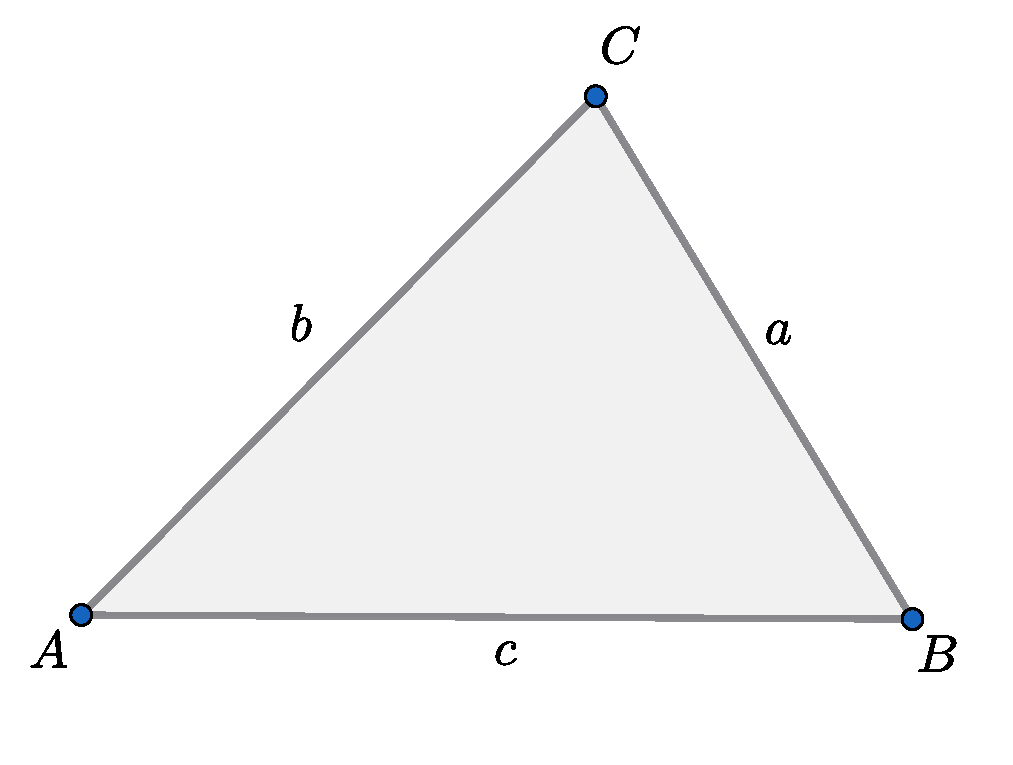
\includegraphics[scale=0.4]{25}
    	\caption{}
       \label{Figure25}
\end{figure} 
\begin{theorembox}[กฏของไซน์]
กำหนดให้ $\triangle ABC$ ถูกล้อมรอบด้วยวงกลมรัศมี $R$ แต่มีความยาวแต่ละด้านซึ่งแสดงดังรูปที่~\ref{Figure26} เราจะได้ความสัมพันธ์ว่า
\[\frac{a}{\sin(A)}=\frac{b}{\sin(B)}=\frac{c}{\sin(C)}=2R\]
\end{theorembox}
 \begin{figure}[H]	 
	\centering
	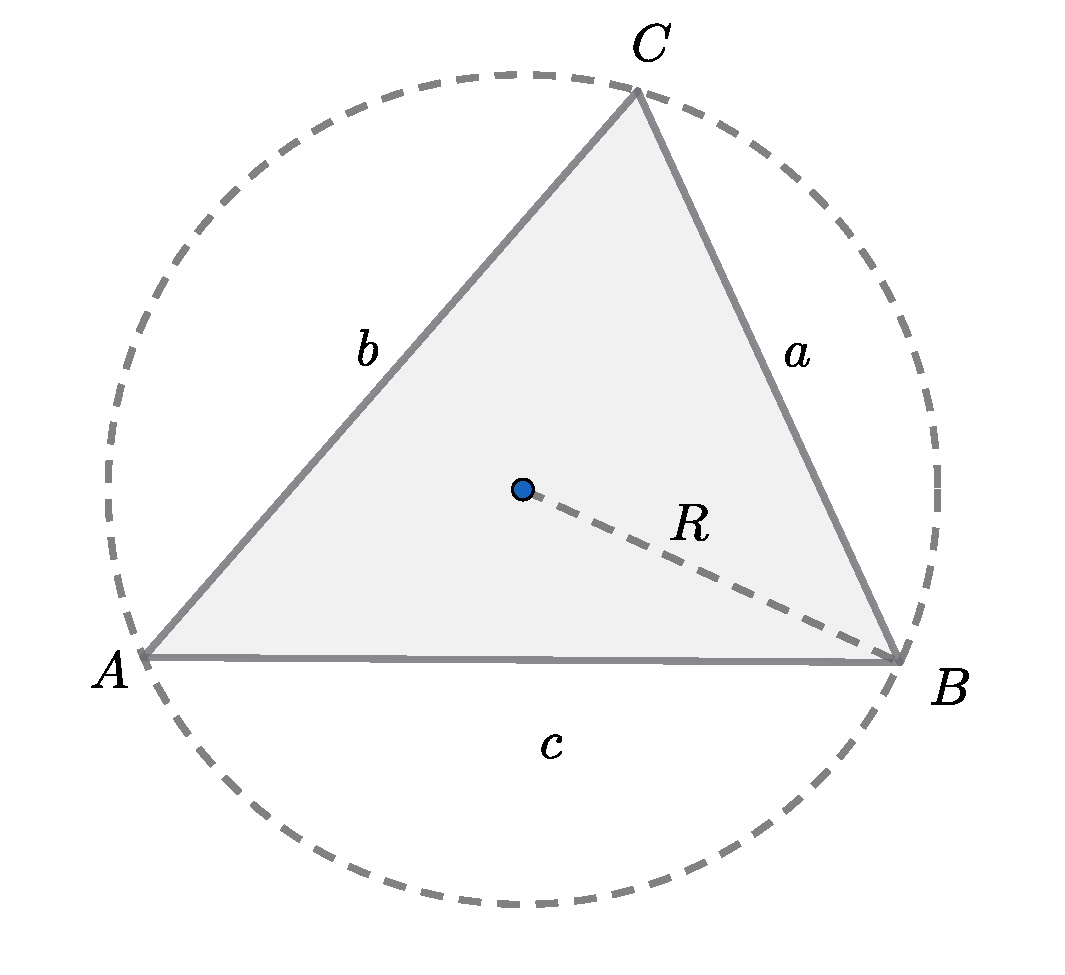
\includegraphics[scale=0.4]{26}
    	\caption{}
       \label{Figure26}
\end{figure} 

\newpage
\begin{examplebox}[NETSAT คณิตศาสตร์ สิงหาคม 2568]  
กำหนดให้ $\triangle ABC$ มี $AB=3$ หน่วย $AC=3$ หน่วย และ $\angle A =120^{\circ}$ จงหาความยาวด้าน $BC$
\begin{enumerate}
\item $3\sqrt{3}$
\item $3\sqrt{5}$
\item $3\sqrt{7}$
\item $9$
\end{enumerate}
\end{examplebox}

\begin{examplebox}[NETSAT คณิตศาสตร์ 2566]
จากรูปที่~\ref{Figure27} จงหาขนาดของมุม $B$
\begin{enumerate}
\item $30^{\circ}$
\item $45^{\circ}$
\item $60^{\circ}$
\item $75^{\circ}$
\end{enumerate}
\end{examplebox} 
\begin{figure}[H]	 
	\centering
	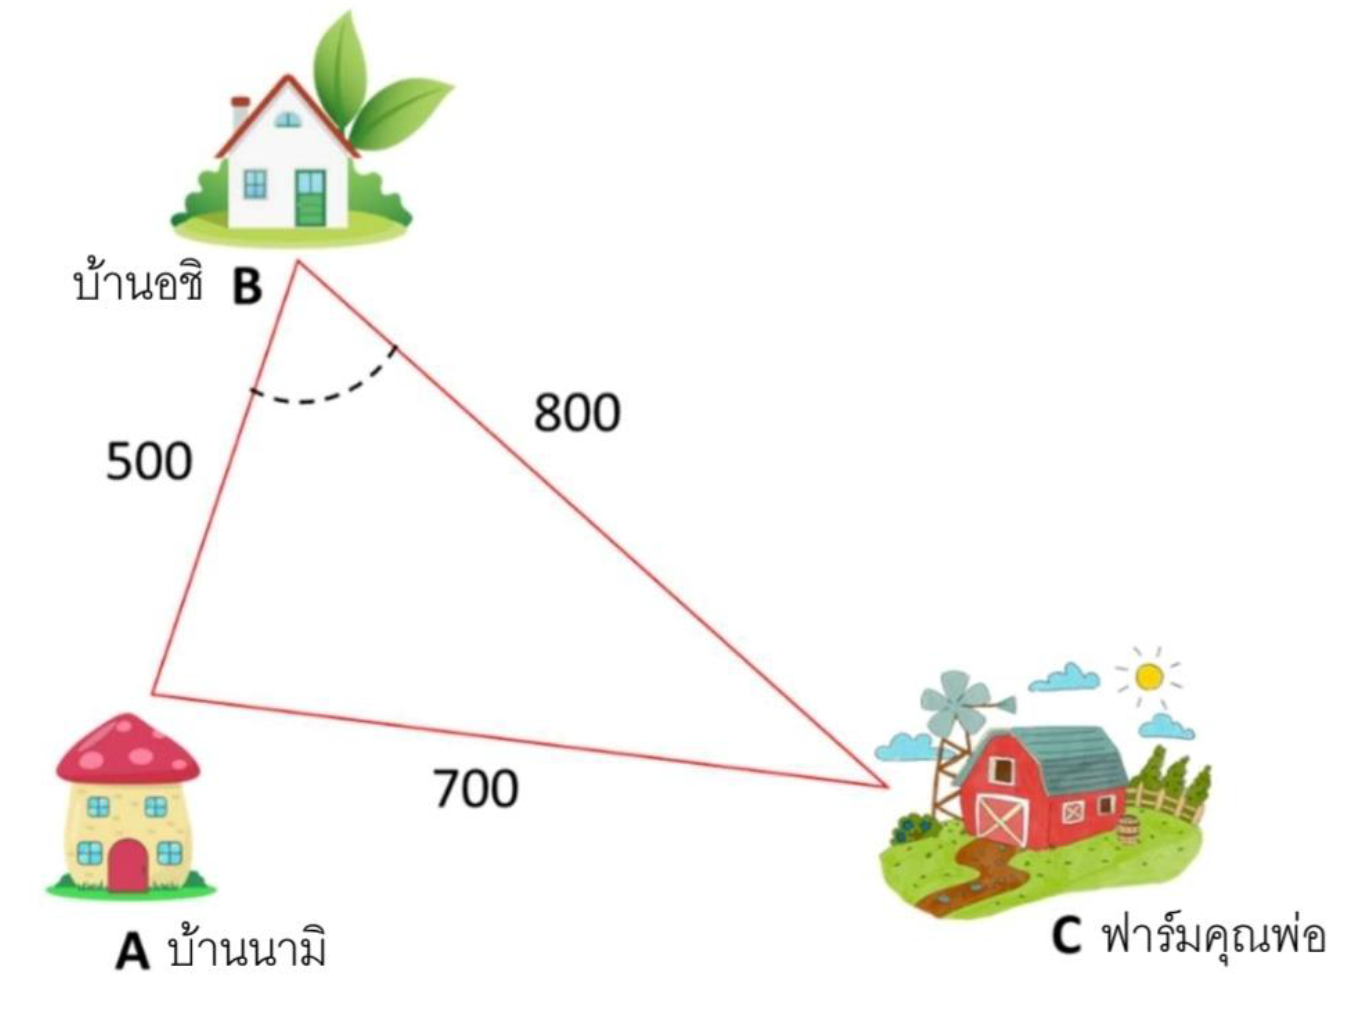
\includegraphics[scale=0.6]{27}
    	\caption{}
       \label{Figure27}
\end{figure} 

\newpage
\begin{examplebox}[NETSAT คณิตศาสตร์ 2566]
รูปที่~\ref{Figure28} แสดงภาพมุมสูงของม้าหมุนในสวน แห่งหนึ่ง โดยมีที่นั่งอยู่บนเส้นรอบวงสองวง และ หมุนรอบจุดศูนย์กลาง $O$ โดยมีรัศมีของวงกลมด้าน นอกเท่ากับ $10$ เมตร รัศมีของวงกลมด้านในเท่ากับ $6$ เมตร
กำหนดให้ที่นั่ง $A$ และ $B$ อยู่ข้างกันบนเส้นรอบวงด้าน นอก และด้านในตามลำดับ โดยไม่คำนึงขนาดของที่นั่ง เมื่อที่นั่ง $A$ และ $B$ เริ่มขยับไปพร้อมๆ กัน รูปที่ 2 แสดงให้เห็นตำแหน่ง $A$ และ $B$ หลังผ่านไป $2-3$ นาที หลังจากเริ่มหมุน ถ้า $\angle AOB=\theta$ และ $\cos(\theta)=\dfrac{11}{24}$ จงหาระยะทางจาก $A$ มา $B$
\begin{enumerate}
\item $7$
\item $9$
\item $11$
\item $13$
\end{enumerate}
\end{examplebox} 
\begin{figure}[H]	 
	\centering
	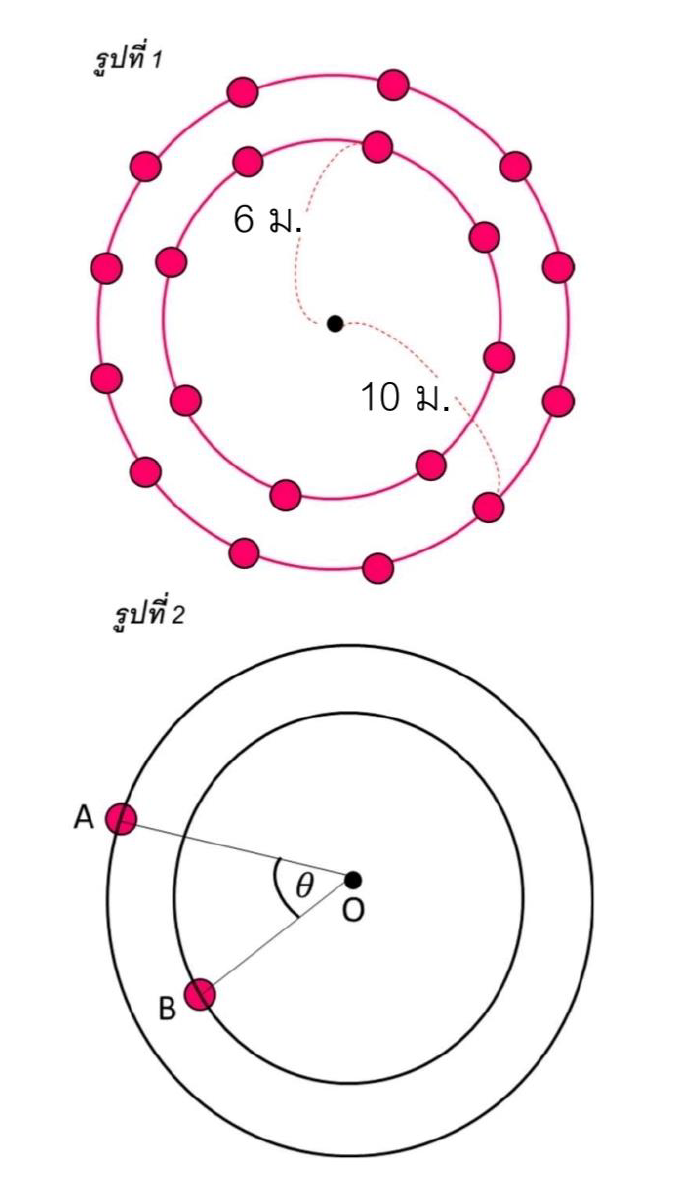
\includegraphics[scale=0.7]{28}
    	\caption{}
       \label{Figure28}
\end{figure}	
	\chapter{ทบทวนความรู้พื้นฐานเรื่องเซต}
\section{การดำเนินการทางเซต}
กำหนดให้ $\mathcal{U}$ แทนเอกภพสัมพัทธ์ และให้ $A,B$ เป็นเซตย่อยของ $\mathcal{U}$
\subsection{ยูเนียน}
\noindent
ให้ $A$ และ $B$ เป็นเซต  
\textbf{ยูเนียนของเซต $A$ และ $B$} แทนด้วยสัญลักษณ์ $A \cup B$  
หมายถึง เซตของสมาชิกทั้งหมดที่อยู่ในเซต $A$ หรือเซต $B$ หรืออยู่ในทั้งสองเซตร่วมกัน

\begin{examplebox}\label{example2.1}
\begin{align*}
\{1,2,3\} \cup \{2,3,4\} &= \{1,2,3,4\}\\
\{3,5\} \cup \{2,3,5\} &= \{2,3,5\}\\
\{1,3,5\} \cup \{2,4,6\} &= \{1,2,3,4,5,6\} \\
\{1,2\} \cup \varnothing &= \{1,2\}
\end{align*}
\end{examplebox}

จากตัวอย่าง~\ref{example2.1} จะได้สมบัติที่สำคัญคือ  
\[
A \cup \varnothing = A 
\quad \text{และ} \quad 
A \cup \mathcal{U} = \mathcal{U}
\]

\newpage
\subsection{อินเตอร์เซก}
\noindent
ให้ $A$ และ $B$ เป็นเซต  
\textbf{อินเตอร์เซกของเซต $A$ และ $B$} แทนด้วยสัญลักษณ์ $A \cap B$  
หมายถึง เซตของสมาชิกที่อยู่ร่วมกันในทั้งเซต $A$ และเซต $B$

\begin{examplebox}\label{example2.2}
\begin{align*}
\{1,2,3\} \cap \{2,3,4\} &= \{2,3\}\\
\{3,5\} \cap \{2,3,5\} &= \{3,5\}\\
\{1,3,5\} \cap \{2,4,6\} &= \varnothing \\
\{1,2\} \cap \varnothing &= \varnothing
\end{align*}
\end{examplebox}

จากตัวอย่าง~\ref{example2.2} จะได้สมบัติว่า  
\[
A \cap \varnothing = \varnothing 
\quad \text{และ} \quad 
A \cap \mathcal{U} = A
\]


\subsection{ผลต่างของเซต}
\noindent
ให้ $A$ และ $B$ เป็นเซต  
\textbf{ผลต่างของเซต $A$ กับ $B$} แทนด้วยสัญลักษณ์ $A-B$  
หมายถึง เซตของสมาชิกที่อยู่ในเซต $A$ แต่ไม่อยู่ในเซต $B$

\begin{examplebox}\label{example2.3}
\begin{align*}
\{1,2,3\}-\{2,3,4\} &= \{1\}\\  
\{7,8,9\}-\{8\} &= \{7,9\} \\
\{1,3,5\}-\{2,4,6\} &= \{1,3,5\}\\
\{2,3,4\}-\{1,2,3\} &= \{4\} \\
\{3,5\}-\{2,3,5\} &= \varnothing \\
\{1,2\}-\varnothing &= \{1,2\}
\end{align*}
\end{examplebox}

จากตัวอย่าง~\ref{example2.3} จะได้ว่า  
\[
A-\varnothing = A 
\quad \text{และ} \quad 
A-\mathcal{U} = \varnothing
\]

\newpage
\subsection{คอมพลีเมนต์ของเซต}
\noindent
ให้ $A$ เป็นเซตย่อยของเอกภพสัมพัทธ์ $\mathcal{U}$  
\textbf{คอมพลีเมนต์ของเซต $A$} แทนด้วยสัญลักษณ์ $A^{\prime}$ หรือ $A^c$  
หมายถึง เซตของสมาชิกทั้งหมดใน $\mathcal{U}$ ที่ไม่อยู่ในเซต $A$

กล่าวคือ
\[
A^{\prime} = A^c = \mathcal{U}-A
\]

\begin{examplebox}\label{example2.4}
กำหนดให้ $\mathcal{U}=\{1,2,3,4,5\}$
\begin{align*}
\{1,2,3\}^c &= \{4,5\}\\  
\{1,4\}^c &= \{2,3,5\}\\ 
\mathcal{U}^c &= \varnothing\\ 
\varnothing^c &= \mathcal{U}
\end{align*}
\end{examplebox}

จากตัวอย่าง~\ref{example2.4} จะเห็นว่า  
\[
\mathcal{U}^c=\varnothing 
\quad \text{และ} \quad 
\varnothing^c=\mathcal{U}
\]

\newpage
\begin{examplebox}[NETSAT คณิตศาสตร์ สิงหาคม 2565]
กำหนดให้ $A=\{1,3,5,7,9\}$ และ $B=\{2,3,4,5,6\}$  
ข้อใดถูกต้อง
\begin{enumerate}
\item $A \cap B=\{3,5\}$
\item $A \cup B$ มีจำนวนสมาชิก $10$ ตัว
\item $A-B=B-A$
\item ถูกต้องทั้งข้อ 1, 2 และ 3
\end{enumerate}
\end{examplebox}

\newpage
\begin{examplebox}[NETSAT คณิตศาสตร์ 2566]
กำหนดให้ $A=\{1,3,4,8\}$ และ $B=\{2,3,5,8,9\}$  
ข้อใดถูกต้อง
\begin{enumerate}
\item $A-B=B-A$
\item $A \cup B$ มีจำนวนสมาชิก $9$ ตัว
\item $A \cap B=\{3,8\}$
\item ถูกต้องทั้งข้อ 1, 2 และ 3
\end{enumerate}
\end{examplebox}

\newpage
\begin{remarkbox}[หลักการรวมเข้า–เอาออก]
ให้ $A,B$ และ $C$ เป็นเซตจำกัด โดยมีจำนวนสมาชิกเท่ากับ $n(A), n(B)$ และ $n(C)$ ตามลำดับ
\begin{itemize}
\item $n(A\cup B)=n(A)+n(B)-n(A\cap B)$
\item $n(A\cup B\cup C)=n(A)+n(B)+n(C)-n(A\cap B)-n(B\cap C)-n(C\cap A)+n(A\cap B\cap C)$
\end{itemize}
\end{remarkbox}


\begin{examplebox}[NETSAT คณิตศาสตร์ สิงหาคม 2568]
มีนักเรียน $50$ คน เลือกเข้าชมรม $3$ ชมรม คือ ดนตรี ศิลปะ และกีฬา  
โดยนักเรียนแต่ละคนต้องเลือกอย่างน้อย $1$ ชมรม แต่ไม่เกิน $2$ ชมรม และมีเงื่อนไขดังนี้
\begin{itemize}
\item จำนวนนักเรียนที่เลือกชมรม $2$ ชมรมใด ๆ มีจำนวนเท่ากัน
\item นักเรียนที่เลือกกีฬามี $20$ คน
\item นักเรียนที่เลือกศิลปะมี $15$ คน
\item นักเรียนที่เลือกศิลปะเพียงชมรมเดียวมี $7$ คน
\end{itemize}
จงหาจำนวนนักเรียนที่เลือกกีฬาเพียงชมรมเดียว
\end{examplebox}
	
	\chapter{ทบทวนความรู้พื้นฐานเรื่องจำนวนจริง}
\section{พหุนาม}
\subsection{การดำเนินการเกี่ยวกับพหุนาม}
\begin{conceptbox}[การบวกและการลบพหุนาม]
\textbf{การบวกและการลบพหุนาม}  
ให้บวกลบเฉพาะเอกนามที่เป็นชนิดเดียวกัน (มีตัวแปรและเลขชี้กำลังเท่ากัน)  
หากไม่สามารถบวกลบกันได้ ให้คงรูปเดิมไว้ เช่น
\begin{align*}
\left(2x^5+4x+5\right)+\left(x^5-x^2-2x\right)
&=3x^5-x^2+2x+5\\
\left(x^2-2x-1\right)-\left(2x^2-x-2\right)
&=-x^2-x+1\\
\left(3x^3-5x+2\right)+\left(-x^3+4x-7\right)
&=2x^3-x-5\\
\left(4x^2+x-6\right)-\left(x^2-3x+1\right)
&=3x^2+4x-7
\end{align*}
\end{conceptbox}

\begin{conceptbox}[การคูณพหุนาม]
\textbf{การคูณพหุนาม}  
ให้ใช้สมบัติการแจกแจง โดยคูณทุกพจน์ของพหุนามหนึ่งเข้ากับทุกพจน์ของอีกพหุนามหนึ่ง เช่น
\begin{align*}
6\left(x^2-x-1\right)
&=6x^2-6x-6\\
\left(x+3\right)\left(x^2-2x+1\right)
&=x^3+x^2-5x+3\\
\left(2x-1\right)\left(x^2+4x-3\right)
&=2x^3+7x^2-10x+3
\left(2x^2+4x+5\right)\left(x^2-2\right)\\
&=2x^4-4x^2+4x^3-8x+5x^2-10\\
&=2x^4+4x^3+x^2-8x-10\\
\end{align*}
\end{conceptbox}

\newpage

\begin{examplebox}[NETSAT คณิตศาสตร์ 2566]
กำหนด $A=-9 x^2+4 x+2$ และ $B=3 x^2+x-7$ ข้อใดต่อไปนี้ถูกต้อง
\begin{enumerate}
\item $2 A-B=-15 x^2-3 x-5$
\item $2 A-3 B=-21 x^2+24 x-17$
\item $A+3 B=7 x-19$
\item ไม่ถูกต้องทั้งข้อ 1, 2 และ 3
\end{enumerate}
\end{examplebox}

\newpage
\begin{examplebox}[NETSAT คณิตศาสตร์ 2566]
ข้อใดต่อไปนี้คือการกระจายนิพจน์ $x(x-8)-(x+2)(x-3)$ และทำให้อยู่ในรูปอย่างง่าย
\begin{enumerate}
\item $-7 x+6$
\item $-9 x+6$
\item $-10 x+6$
\item ถูกต้องทั้งข้อ 1, 2 และ 3
\end{enumerate}
\end{examplebox}

\newpage
\begin{examplebox}[NETSAT คณิตศาสตร์ 2566]
ข้อใดต่อไปนี้คือการแยกตัวประกอบของ $5 x+2 y-x y-10$
\begin{enumerate}
\item $(y-2)(5-x)$
\item $(x-2)(5-y)$
\item $(x-2)(y+5)$
\item $(y-5)(x+2)$
\end{enumerate}
\end{examplebox}

\newpage
\begin{remarkbox}[สูตรการกระจายที่ควรรู้]
\begin{itemize}
    \item[*] $(a+b)^2=a^2+2ab+b^2$
    \item[*] $(a-b)^2=a^2-2ab+b^2$
    \item[*] $(a+b)^3=a^3+3a^2b+3ab^2+b^3$
    \item[*] $(a-b)^3=a^3-3a^2b+3ab^2-b^3$
    \item[*] $a^2-b^2=(a+b)(a-b)$
    \item[*] $a^3+b^3=(a+b)(a^2-ab+b^2)$
    \item[*] $a^3-b^3=(a-b)(a^2+ab+b^2)$
\end{itemize}   
\end{remarkbox}

\begin{examplebox}[NETSAT คณิตศาสตร์ กุมภาพันธ์ 2565]
การกระจายนิพจน์ในข้อใดถูกต้อง
\begin{enumerate}
\item $(x-2)^2+x(x+4)=2 x^2+4$
\item $(x+4)^2-x(x-1)=7 x+16$
\item $4(x-1)^2+(x+2)^2=3 x^2-4 x$
\item ถูกต้องทั้งข้อ 1, 2 และ 3
\end{enumerate}
\end{examplebox}
\newpage
\begin{examplebox}[NETSAT คณิตศาสตร์ กุมภาพันธ์ 2565]
การแยกตัวประกอบของนิพจน์ในข้อใดถูกต้อง
\begin{enumerate}
\item $100 x^2-49 y^2=(10 x+7 y)(10 x-7 y)$
\item $27 x^3+125 y^3=(3 x+5 y)\left(9 x^2-15 x y+25 y^2\right)$
\item $x^3-12 x^2 y+48 x y^2-64 y^3=(x-4 y)^3$
\item ถูกต้องทั้งข้อ 1, 2 และ 3
\end{enumerate}
\end{examplebox}
\newpage
\begin{examplebox}[NETSAT คณิตศาสตร์ 2566]
ข้อใดต่อไปนี้คือการแยกตัวประกอบของนิพจน์ $25 x^2-81 y^2$
\begin{enumerate}
\item $(5 x-9 y)(5 x+9 y)$
\item $(5 x-81 y)(5 x+y)$
\item $(25 x-9 y)(x+9 y)$
\item ถูกต้องทั้งข้อ 1, 2 และ 3
\end{enumerate}
\end{examplebox}
\newpage
\begin{examplebox}[NETSAT คณิตศาสตร์ 2566]
ข้อใดต่อไปคือการกระจายพจน์ $(4 x-3 y)^3$ และทำให้อยู่ในรูปอย่างง่าย
\begin{enumerate}
\item $64 x^3-144 x^2 y+108 x y^2-27 y^3$
\item $64 x^3+144 x^2 y-108 x y^2-27 y^3$
\item $64 x^3-108 x^2 y+144 x y^2-27 y^3$
\item $64 x^3+108 x^2 y-144 x y^2+27 y^3$
\end{enumerate}
\end{examplebox}

\newpage
\begin{examplebox}[NETSAT คณิตศาสตร์ กุมภาพันธ์ 2567]
ข้อใดถูกต้อง
\begin{enumerate}
\item $(x+3)\left(x^2-3 x+9\right)=x^3-27$
\item $(x+3)(x+2)(x-2)(x-3)=x^4-25 x^2+36$
\item $(x+5)^2-(x+3)(x-3)=10 x+16$
\item $(x+3)(x-2)-x(x+1)=-6$
\end{enumerate}
\end{examplebox}

\newpage
\begin{examplebox}[NETSAT คณิตศาสตร์ กุมภาพันธ์ 2567]
ข้อใดต่อไปนี้แยกตัวประกอบได้ถูกต้อง
\begin{multicols}{2}
\begin{enumerate}
\item $a x^2-8 a x+16 a=a(x-4)^2$
\item $a^2+7 a+12=(a+4)(a+3)$
\item $a b-a-b+1=(a-1)(b-1)$
\item ถูกต้องทั้งข้อ 1, 2 และ 3
\end{enumerate}
\end{multicols}
\end{examplebox}
\newpage
\subsection{การหารสังเคราะห์}
\begin{examplebox}
จงใช้การหารสังเคราะห์เพื่อหาผลหารและเศษ จาการหารพหุนาม $3x^4+2x^2+3x-5$ ด้วย $x+1$
\end{examplebox}
\vspace{10cm}
\begin{examplebox}
จงใช้การหารสังเคราะห์เพื่อหาผลหารและเศษ จาการหารพหุนาม $x^3+x^2-18x+18$ ด้วย $x-3$
\end{examplebox}

\newpage
\begin{examplebox}
กำหนดให้ $p(x)=x^4-3x^3-5x^2+x-8$ และ $q(x)=x^2+4x-2$ จงใช้การหารสังเคราะห์เพื่อหาผลหารและเศษ จาการหารพหุนาม $p(x)$ ด้วย $q(x)$
\end{examplebox}

\newpage
\subsection{ทฤษฎีบทเศษเหลือ}
\begin{theorembox}
กำหนดให้ $p(x)$ เป็นพหุนาม และ $\alpha$ เป็นจำนวนจริง  
เมื่อหารพหุนาม $p(x)$ ด้วยพหุนาม $x-\alpha$ แล้ว  
\textbf{เศษจากการหารจะมีค่าเท่ากับ $p(\alpha)$}
\end{theorembox}

\begin{examplebox}
จงใช้ทฤษฎีบทเศษเหลือหาเศษเหลือจาการหารพหุนาม $x^4-5x^3+2x^2-x+2$ ด้วย $x-3$
\end{examplebox}
\vspace{3cm}
\begin{examplebox}
จงใช้ทฤษฎีบทเศษเหลือหาเศษเหลือจาการหารพหุนาม $x^3-x^2-x-15$ ด้วย $x-3$
\end{examplebox}
\vspace{3cm}
\begin{examplebox}
กำหนดพหุนาม $p(x)=x^3+6x^2-2\alpha x-3$ และ $q(x)=x^2+4x-2$ จงหาจำนวนจริง $\alpha$ ที่ทำให้ $p(x)$ ถูกหารด้วยพหุนาม $x+3$ ลงตัว
\end{examplebox}

\newpage
\begin{remarkbox}
กำหนดให้ $p(x)$ เป็นพหุนาม และ $\alpha$ เป็นจำนวนจริง
\begin{itemize}
    \item $p(\alpha)=0$ ก็ต่อเมื่อ พหุนาม $x-\alpha$ เป็นตัวประกอบของพหุนาม $p(x)$
    \item ถ้า $p(\alpha)=0$ จะเรียก $\alpha$ ว่า \textbf{ราก} หรือ \textbf{คำตอบ} ของพหุนาม $p(x)$  และของสมการ $p(x)=0$
\end{itemize}
\end{remarkbox}


\begin{examplebox}[NETSAT คณิตศาสตร์ กุมภาพันธ์ 2565]
ถ้าพหุนาม $x^3-x^2+a x+4$ ถูกหารลงตัวด้วย $x+2$ แล้ว $a$ มีค่าเท่าไร
\begin{multicols}{2}
\begin{enumerate}
\item $-2$
\item $2$
\item $-4$
\item $4$
\end{enumerate}
\end{multicols}
\end{examplebox}

\vspace{6cm}
\begin{examplebox}[NETSAT คณิตศาสตร์ กุมภาพันธ์ 2567]
ข้อใดคือเศษที่ได้จากการหารพหนุนามด้วย $3 x^3+4 x^2-6 x-10$ ด้วย $x-2$
\begin{multicols}{2}
\begin{enumerate}
\item $-6x^2$
\item $6 x$
\item $-6$
\item $6$
\end{enumerate}
\end{multicols}
\end{examplebox}

\newpage
\section{สมการตัวแปรเดียว $ax^2+bx+c=0$ เมื่อ $a\neq 0$}
\begin{theorembox}
สมการกำลังสองตัวแปรเดียว
\[
ax^2+bx+c=0 \quad (a\neq 0)
\]
จะมีคำตอบในระบบจำนวนจริงได้ไม่เกินสองคำตอบ  
โดยพิจารณาจากค่าของตัวแยกกำลังสอง (discriminant) คือ $b^2-4ac$ ดังนี้
\begin{itemize}
    \item ถ้า $b^2-4ac>0$ สมการจะมีคำตอบจริง \textbf{สองคำตอบที่แตกต่างกัน}
    \item ถ้า $b^2-4ac=0$ สมการจะมีคำตอบจริง \textbf{เพียงหนึ่งคำตอบ}
    \item ถ้า $b^2-4ac<0$ สมการจะ \textbf{ไม่มีคำตอบในระบบจำนวนจริง}
\end{itemize}
และคำตอบของสมการสามารถเขียนในรูป
\[
x=\dfrac{-b\pm\sqrt{b^2-4ac}}{2a}
\]
\end{theorembox}

\subsection{ผลบวกรากและผลคูณรากของสมการ $ax^2+bx+c=0$ เมื่อ $a\neq 0$}
\begin{remarkbox}
ถ้าสมการ $ax^2+bx+c=0$ มี $\alpha$ และ $\beta$ เป็นคำตอบ  
(อาจเป็นคำตอบซ้ำหรือคำตอบที่แตกต่างกัน) แล้วจะมีความสัมพันธ์ดังนี้
\begin{align*}
 \alpha+\beta &=-\dfrac{b}{a}\\
 \alpha\beta &=\dfrac{c}{a}
\end{align*}
\end{remarkbox}


\begin{examplebox}[NETSAT คณิตศาสตร์ กุมภาพันธ์ 2565]
ให้ $a$ และ $b$ เป็นคำตอบของสมการ $x^2+2 x-6=0$ ข้อใดถูกต้อง
\begin{multicols}{2}
\begin{enumerate}
\item $a+b=-2$
\item $(a-b)^2=28$
\item $a b=-6$
\item ถูกต้องทั้งข้อ 1, 2 และ 3
\end{enumerate}
\end{multicols}
\end{examplebox}

\newpage
\begin{examplebox}[NETSAT คณิตศาสตร์ สิงหาคม 2565]
ให้ $x=a$ และ $x=b$ เป็นคำตอบของสมการ $x^2+2 x-2=0$ ข้อใดต่อไปนี้ถูกต้อง
\begin{multicols}{2}
\begin{enumerate}
\item $a-b=2 \sqrt{3}$
\item $a+b=-2$
\item $a b=2$
\item ถูกต้องทั้งข้อ 1, 2 และ 3
\end{enumerate}
\end{multicols}
\end{examplebox}

\newpage
\begin{examplebox}[NETSAT คณิตศาสตร์ 2566]
ให้ $x=a$ และ $y=b$ เป็นคำตอบของของสมการ $(x+1)^2=7$ ข้อใดต่อไปนี้ถูกต้อง
\begin{multicols}{2}
\begin{enumerate}
\item $a=b$
\item $a+b>0$
\item $a b<0$
\item ถูกต้องทั้งข้อ 1, 2 และ 3
\end{enumerate}
\end{multicols}
\end{examplebox}

\newpage
\begin{examplebox}[NETSAT คณิตศาสตร์ 2566]
กำหนดให้ $x$ คือ คำตอบของสมการ $x^2-2 x-6=0$ ข้อใดต่อไปนี้ถูกต้อง
\begin{multicols}{2}
\begin{enumerate}
\item $x=1 \pm \sqrt{7}$
\item ผลรวมของคำตอบของสมการ คือ $2$
\item สมการนี้ไม่มีคำตอบ
\item ถูกต้องทั้งข้อ 1 และ 2
\end{enumerate}
\end{multicols}
\end{examplebox}
	\chapter{ทบทวนความรู้พื้นฐานเรื่องตรีโกณมิติ}
\section{อัตราส่วนตรีโกณมิติ}
พิจารณาสามเหลี่ยมมุมฉาก $ABC$ ซึ่งมีมุม $C$ เป็นมุมฉาก ดังรูปที่~\ref{Figure50}
\begin{figure}[H] 
\centering 
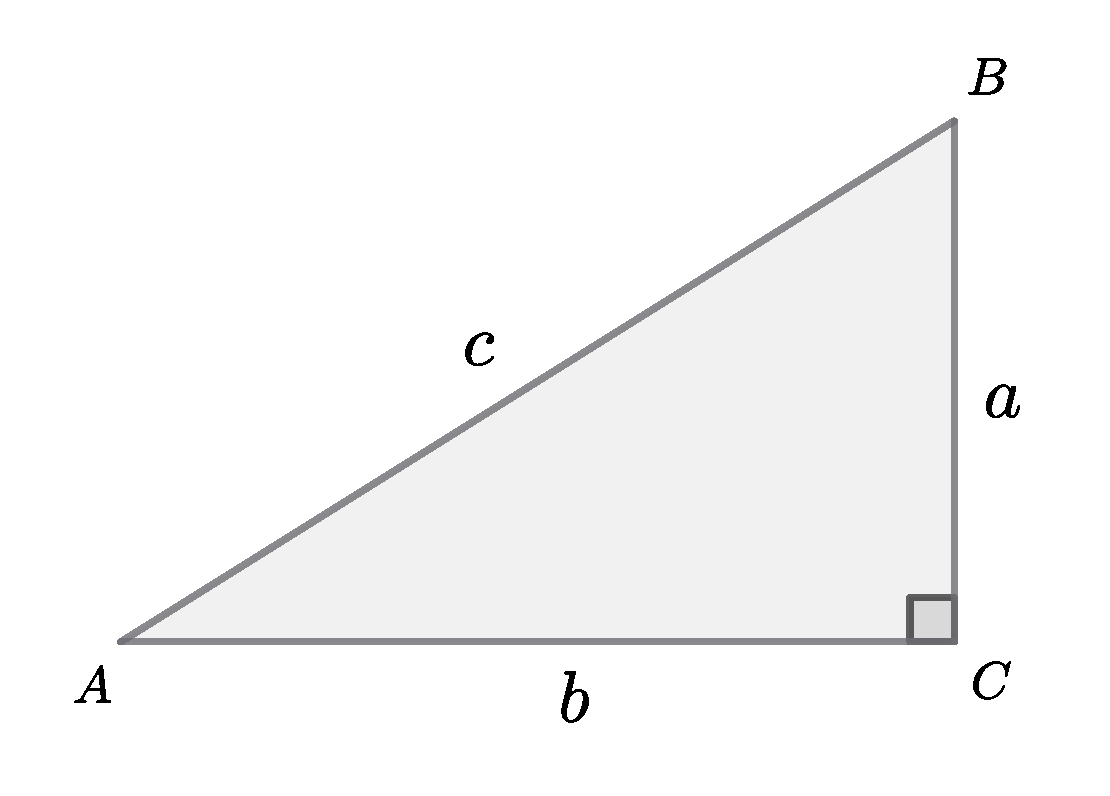
\includegraphics[scale=0.5]{50} 
\caption{} 
\label{Figure50} 
\end{figure}
\begin{itemize}
\item $AB$ เป็น \textbf{ด้านตรงข้ามมุมฉาก} (ด้านยาวที่สุดของสามเหลี่ยม) และมีความยาว $c$ หน่วย
\item $BC$ เป็น \textbf{ด้านตรงข้ามมุม} $A$ และมีความยาว $a$ หน่วย
\item $AC$ เป็น \textbf{ด้านตรงข้ามมุม} $B$ และมีความยาว $b$ หน่วย
\end{itemize}
จากรูปที่~\ref{Figure50} สามารถนิยามอัตราส่วนตรีโกณมิติที่สัมพันธ์กับด้านของสามเหลี่ยมมุมฉากได้ดังต่อไปนี้
\newpage
\begin{remarkbox}
\begin{enumerate}
    \item \textbf{ไซน์ของมุม $A$} แทนด้วยสัญลักษณ์ $\sin(A)$ นิยามโดย
    \[
    \sin(A)=\frac{\text{ความยาวด้านที่อยู่ตรงข้ามมุม } A}{\text{ความยาวด้านตรงข้ามมุมฉาก}}
    =\frac{a}{c}
    \]

    \item \textbf{โคไซน์ของมุม $A$} แทนด้วยสัญลักษณ์ $\cos(A)$ นิยามโดย
    \[
    \cos(A)=\frac{\text{ความยาวด้านประชิดมุม } A}{\text{ความยาวด้านตรงข้ามมุมฉาก}}
    =\frac{b}{c}
    \]

    \item \textbf{แทนเจนต์ของมุม $A$} แทนด้วยสัญลักษณ์ $\tan(A)$ นิยามโดย
    \[
    \tan(A)=\frac{\text{ความยาวด้านที่อยู่ตรงข้ามมุม } A}{\text{ความยาวด้านประชิดมุม } A}
    =\frac{a}{b}
    \]
\end{enumerate}
\end{remarkbox}
\begin{remarkbox}
นอกจากอัตราส่วนตรีโกณมิติพื้นฐานแล้ว ยังมีอัตราส่วนตรีโกณมิติส่วนกลับอีก $3$ อัตราส่วน ดังนี้
\begin{enumerate}
    \item \textbf{โคซีแคนต์ของมุม $A$} แทนด้วยสัญลักษณ์ $\cosec(A)$ ซึ่งเป็นส่วนกลับของ $\sin(A)$
    \[
    \cosec(A)=\frac{1}{\sin(A)} \quad \text{เมื่อ } \sin(A)\neq 0
    \]

    \item \textbf{ซีแคนต์ของมุม $A$} แทนด้วยสัญลักษณ์ $\sec(A)$ ซึ่งเป็นส่วนกลับของ $\cos(A)$
    \[
    \sec(A)=\frac{1}{\cos(A)} \quad \text{เมื่อ } \cos(A)\neq 0
    \]

    \item \textbf{โคแทนเจนต์ของมุม $A$} แทนด้วยสัญลักษณ์ $\cot(A)$ ซึ่งเป็นส่วนกลับของ $\tan(A)$
    \[
    \cot(A)=\frac{1}{\tan(A)} \quad \text{เมื่อ } \tan(A)\neq 0
    \]
\end{enumerate}
\end{remarkbox}


\begin{observationbox}
เนื่องจาก $\sin(A)=\dfrac{a}{c},\,\,\cos(A)=\dfrac{b}{c}$ และ $\tan(A)=\dfrac{a}{b}$\\
\vspace{0.5cm}\\
จะเห็นได้ว่า $\tan(A)=\dfrac{\sin(A)}{\cos(A)}$ และ $\cot(A)=\dfrac{\cos(A)}{\sin(A)}$    
\end{observationbox}

\begin{examplebox}
กำหนดให้ $\triangle ABC$ เป็นสามเหลี่ยมที่มีมุม $C$ เป็นมุมฉาก ถ้า $\cos(A)=\dfrac{3}{5}$ จงหาค่าของ $\sin(A)$ และ $\tan(A)$
\end{examplebox}
\vspace{5cm}
\begin{examplebox}
กำหนดให้ $\triangle ABC$ เป็นสามเหลี่ยมที่มีมุม $C$ เป็นมุมฉาก ถ้า $\tan(A)=\dfrac{5}{12}$ จงหาค่าของ 
\[\dfrac{2\sin(A)+3\cos(A)}{\sin(A)-\cos(A)}\]
\end{examplebox}
\vspace{6cm}
\subsection{ค่าฟังก์ชันตรีโกณมิติของมุมพื้นฐาน}
ตารางต่อไปนี้แสดงค่าฟังก์ชันตรีโกณมิติของมุมพื้นฐานที่ใช้บ่อย ในหน่วยองศา
\begin{table}[h]
\centering
\setlength{\extrarowheight}{4pt}
\begin{tabular}{|c|c|c|c|c|c|c|c|c|}
\hline
$\theta\,(\text{องศา})$ 
& $0^\circ$ 
& $30^\circ$ 
& $45^\circ$ 
& $60^\circ$ 
& $90^\circ$ 
& $180^\circ$
& $270^\circ$
& $360^\circ$\\
\hline

$\sin(\theta)$ 
& $0$ 
& $\dfrac{1}{2}$ 
& $\dfrac{\sqrt{2}}{2}$ 
& $\dfrac{\sqrt{3}}{2}$ 
& $1$ 
& $0$ 
& $-1$ 
& $0$ \\ 
\hline

$\cos(\theta)$ 
& $1$ 
& $\dfrac{\sqrt{3}}{2}$ 
& $\dfrac{\sqrt{2}}{2}$ 
& $\dfrac{1}{2}$ 
& $0$ 
& $-1$ 
& $0$ 
& $1$ \\
\hline

$\tan(\theta)$ 
& $0$ 
& $\dfrac{1}{\sqrt{3}}$ 
& $1$ 
& $\sqrt{3}$ 
& \text{ไม่กำหนดค่า}
& $0$ 
& \text{ไม่กำหนดค่า} 
& $0$ \\
\hline
\end{tabular}
\caption{ค่าฟังก์ชันตรีโกณมิติของมุมพื้นฐานในหน่วยองศา}
\label{table1.1}
\end{table}

\newpage
\section{องศาและเรเดียน}
หน่วยวัดขนาดของมุมที่ใช้กันทั่วไปมี $2$ หน่วย คือ \textbf{องศา} และ \textbf{เรเดียน} 
โดยสามารถแปลงหน่วยระหว่างกันได้ดังนี้
\begin{conceptbox}
 \begin{itemize}
    \item[*] การแปลงจาก \textbf{เรเดียน} เป็น \textbf{องศา} ให้แทน $\pi$ ด้วย $180^\circ$
    \item[*] การแปลงจาก \textbf{องศา} เป็น \textbf{เรเดียน} ให้คูณด้วย $\dfrac{\pi}{180}$
\end{itemize}   
\end{conceptbox}

\begin{examplebox}[NETSAT คณิตศาสตร์ กุมภาพันธ์ 2567]  
$72^{\circ}$ เท่ากับกี่เรเดียน
\begin{multicols}{2}
\begin{enumerate}
\item $\dfrac{2\pi}{3}$
\item $\dfrac{2\pi}{5}$
\item $\dfrac{3\pi}{4}$
\item $\dfrac{3\pi}{5}$
\end{enumerate}
  \end{multicols}
\end{examplebox}

\begin{examplebox}
จงเปลี่ยนมุมพื้นฐานต่อไปนี้ให้อยู่ในหน่วยเรเดียน
\begin{enumerate}
\item $0^\circ$ 
\item $30^\circ$ 
\item $45^\circ$ 
\item $60^\circ$ 
\item $90^\circ$ 
\item $180^\circ$
\item $270^\circ$
\item $360^\circ$
\end{enumerate}
\end{examplebox}

จากตารางที่~\ref{table1.1} สามารถเขียนค่าฟังก์ชันตรีโกณมิติของมุมพื้นฐานในหน่วยเรเดียนได้ดังตารางต่อไปนี้

\begin{table}[h]
\centering
\setlength{\extrarowheight}{4pt}
\begin{tabular}{|c|c|c|c|c|c|c|c|c|}
\hline
$\theta\,(\text{เรเดียน})$ 
& $0$ 
& $\dfrac{\pi}{6}$ 
& $\dfrac{\pi}{4}$ 
& $\dfrac{\pi}{3}$ 
& $\dfrac{\pi}{2}$ 
& $\pi$ 
& $\dfrac{3\pi}{2}$ 
& $2\pi$ \\
\hline

$\sin(\theta)$ 
& $0$ 
& $\dfrac{1}{2}$ 
& $\dfrac{\sqrt{2}}{2}$ 
& $\dfrac{\sqrt{3}}{2}$ 
& $1$ 
& $0$ 
& $-1$ 
& $0$ \\ 
\hline

$\cos(\theta)$ 
& $1$ 
& $\dfrac{\sqrt{3}}{2}$ 
& $\dfrac{\sqrt{2}}{2}$ 
& $\dfrac{1}{2}$ 
& $0$ 
& $-1$ 
& $0$ 
& $1$ \\
\hline

$\tan(\theta)$ 
& $0$ 
& $\dfrac{1}{\sqrt{3}}$ 
& $1$ 
& $\sqrt{3}$ 
& \text{ไม่กำหนดค่า}
& $0$ 
& \text{ไม่กำหนดค่า} 
& $0$ \\
\hline
\end{tabular}
\caption{ค่าฟังก์ชันตรีโกณมิติของมุมพื้นฐานในหน่วยเรเดียน}
\label{table1.2}
\end{table}


\section{ทบทวนสูตรตรีโกณมิติที่จำเป็น}
\subsection{โคฟังก์ชัน}
สำหรับ $0^{\circ}<\theta<90^{\circ}$ จะมีความสัมพันธ์ของโคฟังก์ชันดังนี้
\begin{itemize}
\item $\sin(\theta)=\cos\left(90^\circ-\theta\right)$
\item $\tan(\theta)=\cot\left(90^\circ-\theta\right)$
\item $\sec(\theta)=\cosec\left(90^\circ-\theta\right)$
\end{itemize}

\subsection{เอกลักษณ์ตรีโกณมิติ}
เอกลักษณ์ตรีโกณมิติพื้นฐานที่ใช้บ่อย มีดังนี้
\begin{itemize}
\item $\sin^2(\theta)+\cos^2(\theta)=1$ 
\item $\sec^2(\theta)-\tan^2(\theta)=1$ 
\item $\cosec^2(\theta)-\cot^2(\theta)=1$ 
\end{itemize}

\subsection{ฟังก์ชันตรีโกณมิติของมุมสองเท่า}
ถ้า $\alpha$ เป็นจำนวนจริง จะมีสูตรมุมสองเท่าดังนี้
\begin{itemize}
\item $\sin(2\alpha)=2\sin(\alpha)\cos(\alpha)$
\item $\cos(2\alpha)=\cos^2(\alpha)-\sin^2(\alpha)$
\end{itemize}

\subsection{ฟังก์ชันตรีโกณมิติของผลบวกและผลต่างของมุม}
ให้ $A$ และ $B$ เป็นจำนวนจริง จะได้ว่า
\begin{itemize}
\item $\sin(A+B)=\sin(A)\cos(B)+\cos(A)\sin(B)$ 
\item $\sin(A-B)=\sin(A)\cos(B)-\cos(A)\sin(B)$ 
\item $\cos(A+B)=\cos(A)\cos(B)-\sin(A)\sin(B)$ 
\item $\cos(A-B)=\cos(A)\cos(B)+\sin(A)\sin(B)$
\item $\tan(A+B)=\dfrac{\tan(A)+\tan(B)}{1-\tan(A)\tan(B)}$  
\item $\tan(A-B)=\dfrac{\tan(A)-\tan(B)}{1+\tan(A)\tan(B)}$ 
\end{itemize}

\begin{remarkbox}\label{remark1.3}
สำหรับจำนวนจริง $\theta$ จะมีสมบัติดังนี้
\begin{itemize}
\item $\sin(-\theta)=-\sin(\theta)$
\item $\cos(-\theta)=\cos(\theta)$
\item $\tan(-\theta)=-\tan(\theta)$
\end{itemize}
\end{remarkbox}

\begin{observationbox}\label{observation1.2}
 \begin{enumerate}
     \item $\sin(30^{\circ})=\dfrac{1}{2}$
     \item $\sin\left(\dfrac{\pi}{6}\right)=\dfrac{1}{2}$
 \end{enumerate}
\end{observationbox}
เมื่อมุมมีขนาดมากกว่า $90^{\circ}$ หรือมีค่ามากกว่า $\frac{\pi}{2}$ การหาค่าฟังก์ชันตรีโกณมิติจะไม่สามารถอาศัยตารางมุมพิเศษโดยตรงได้ จึงจำเป็นต้องยุบมุมให้อยู่ในช่วงที่คุ้นเคยก่อน

\begin{observationbox}\label{observation1.3}
 \begin{enumerate}
     \item $\sin(210^{\circ})=?$
     \item $\sin\left(\dfrac{7\pi}{6}\right)=?$
 \end{enumerate}
\end{observationbox}
\newpage
\section{การแปลงมุมในรูปอย่างง่าย}
\subsection{เครื่องหมายและจตุภาค (ควอดรันท์)} \label{section1.4.1}
จากรูปที่~\ref{Figure51} สัญลักษณ์ $Q_1,Q_2,Q_3$ และ $Q_4$ หมายถึง
\textbf{จตุภาคที่หนึ่ง จตุภาคที่สอง จตุภาคที่สาม และจตุภาคที่สี่}
(หรือเรียกว่า \textbf{ควอดรันท์ที่หนึ่ง สอง สาม และสี่}) ตามลำดับ
เราจะได้เครื่องหมายของฟังก์ชันตรีโกณมิติ $\sin$ และ $\cos$
ในแต่ละจตุภาคดังต่อไปนี้

\begin{figure}[H]	 
	\centering
	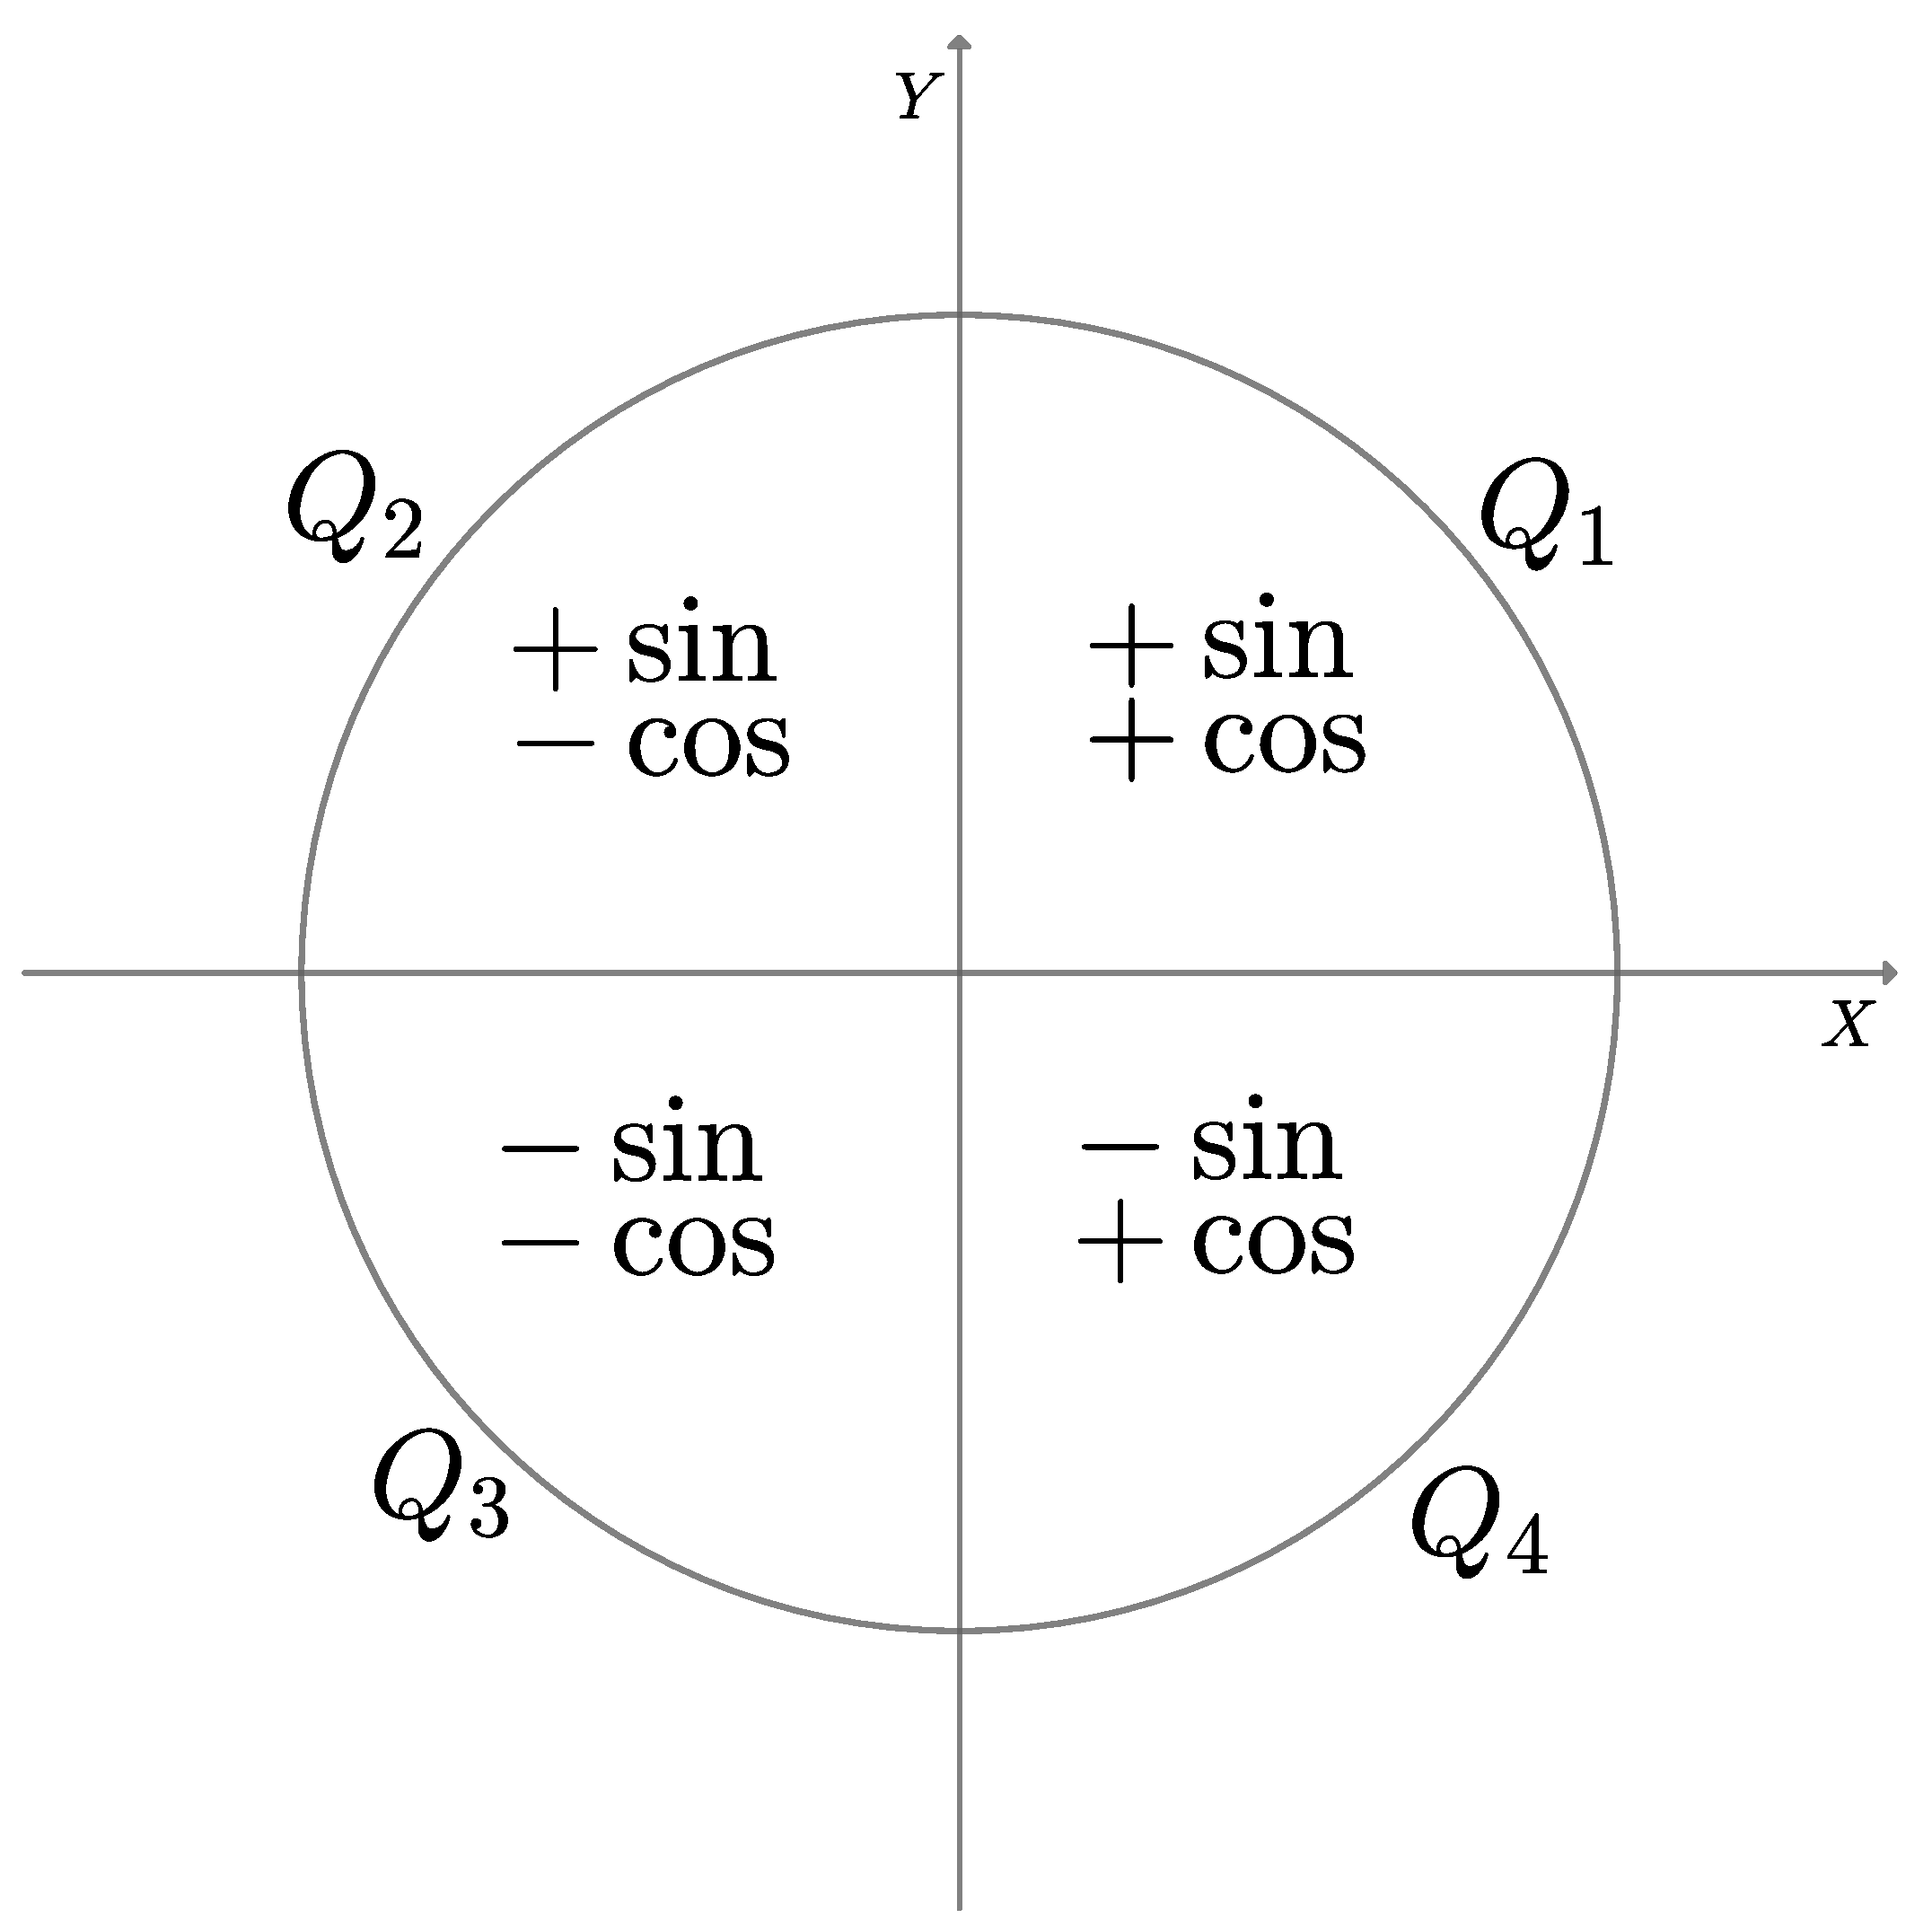
\includegraphics[scale=0.5]{52}
    	\caption{}
       \label{Figure52}
\end{figure} 
\newpage

\begin{examplebox}
ถ้า $\sin(\theta)>0$ และ $\cos(\theta)<0$ แล้ว $\theta$ อยู่ควอดรันท์ใด
\end{examplebox}
\vspace{8cm}

\begin{examplebox}
กำหนดให้ $\tan^2(\theta)=\dfrac{1}{5}$ และ $\theta$ อยู่ควอดรันท์ที่สอง จงหาค่า $\cot(\theta)$
\end{examplebox}

\newpage
\subsection{การวัดมุม}
\begin{figure}[H]	 
	\centering
	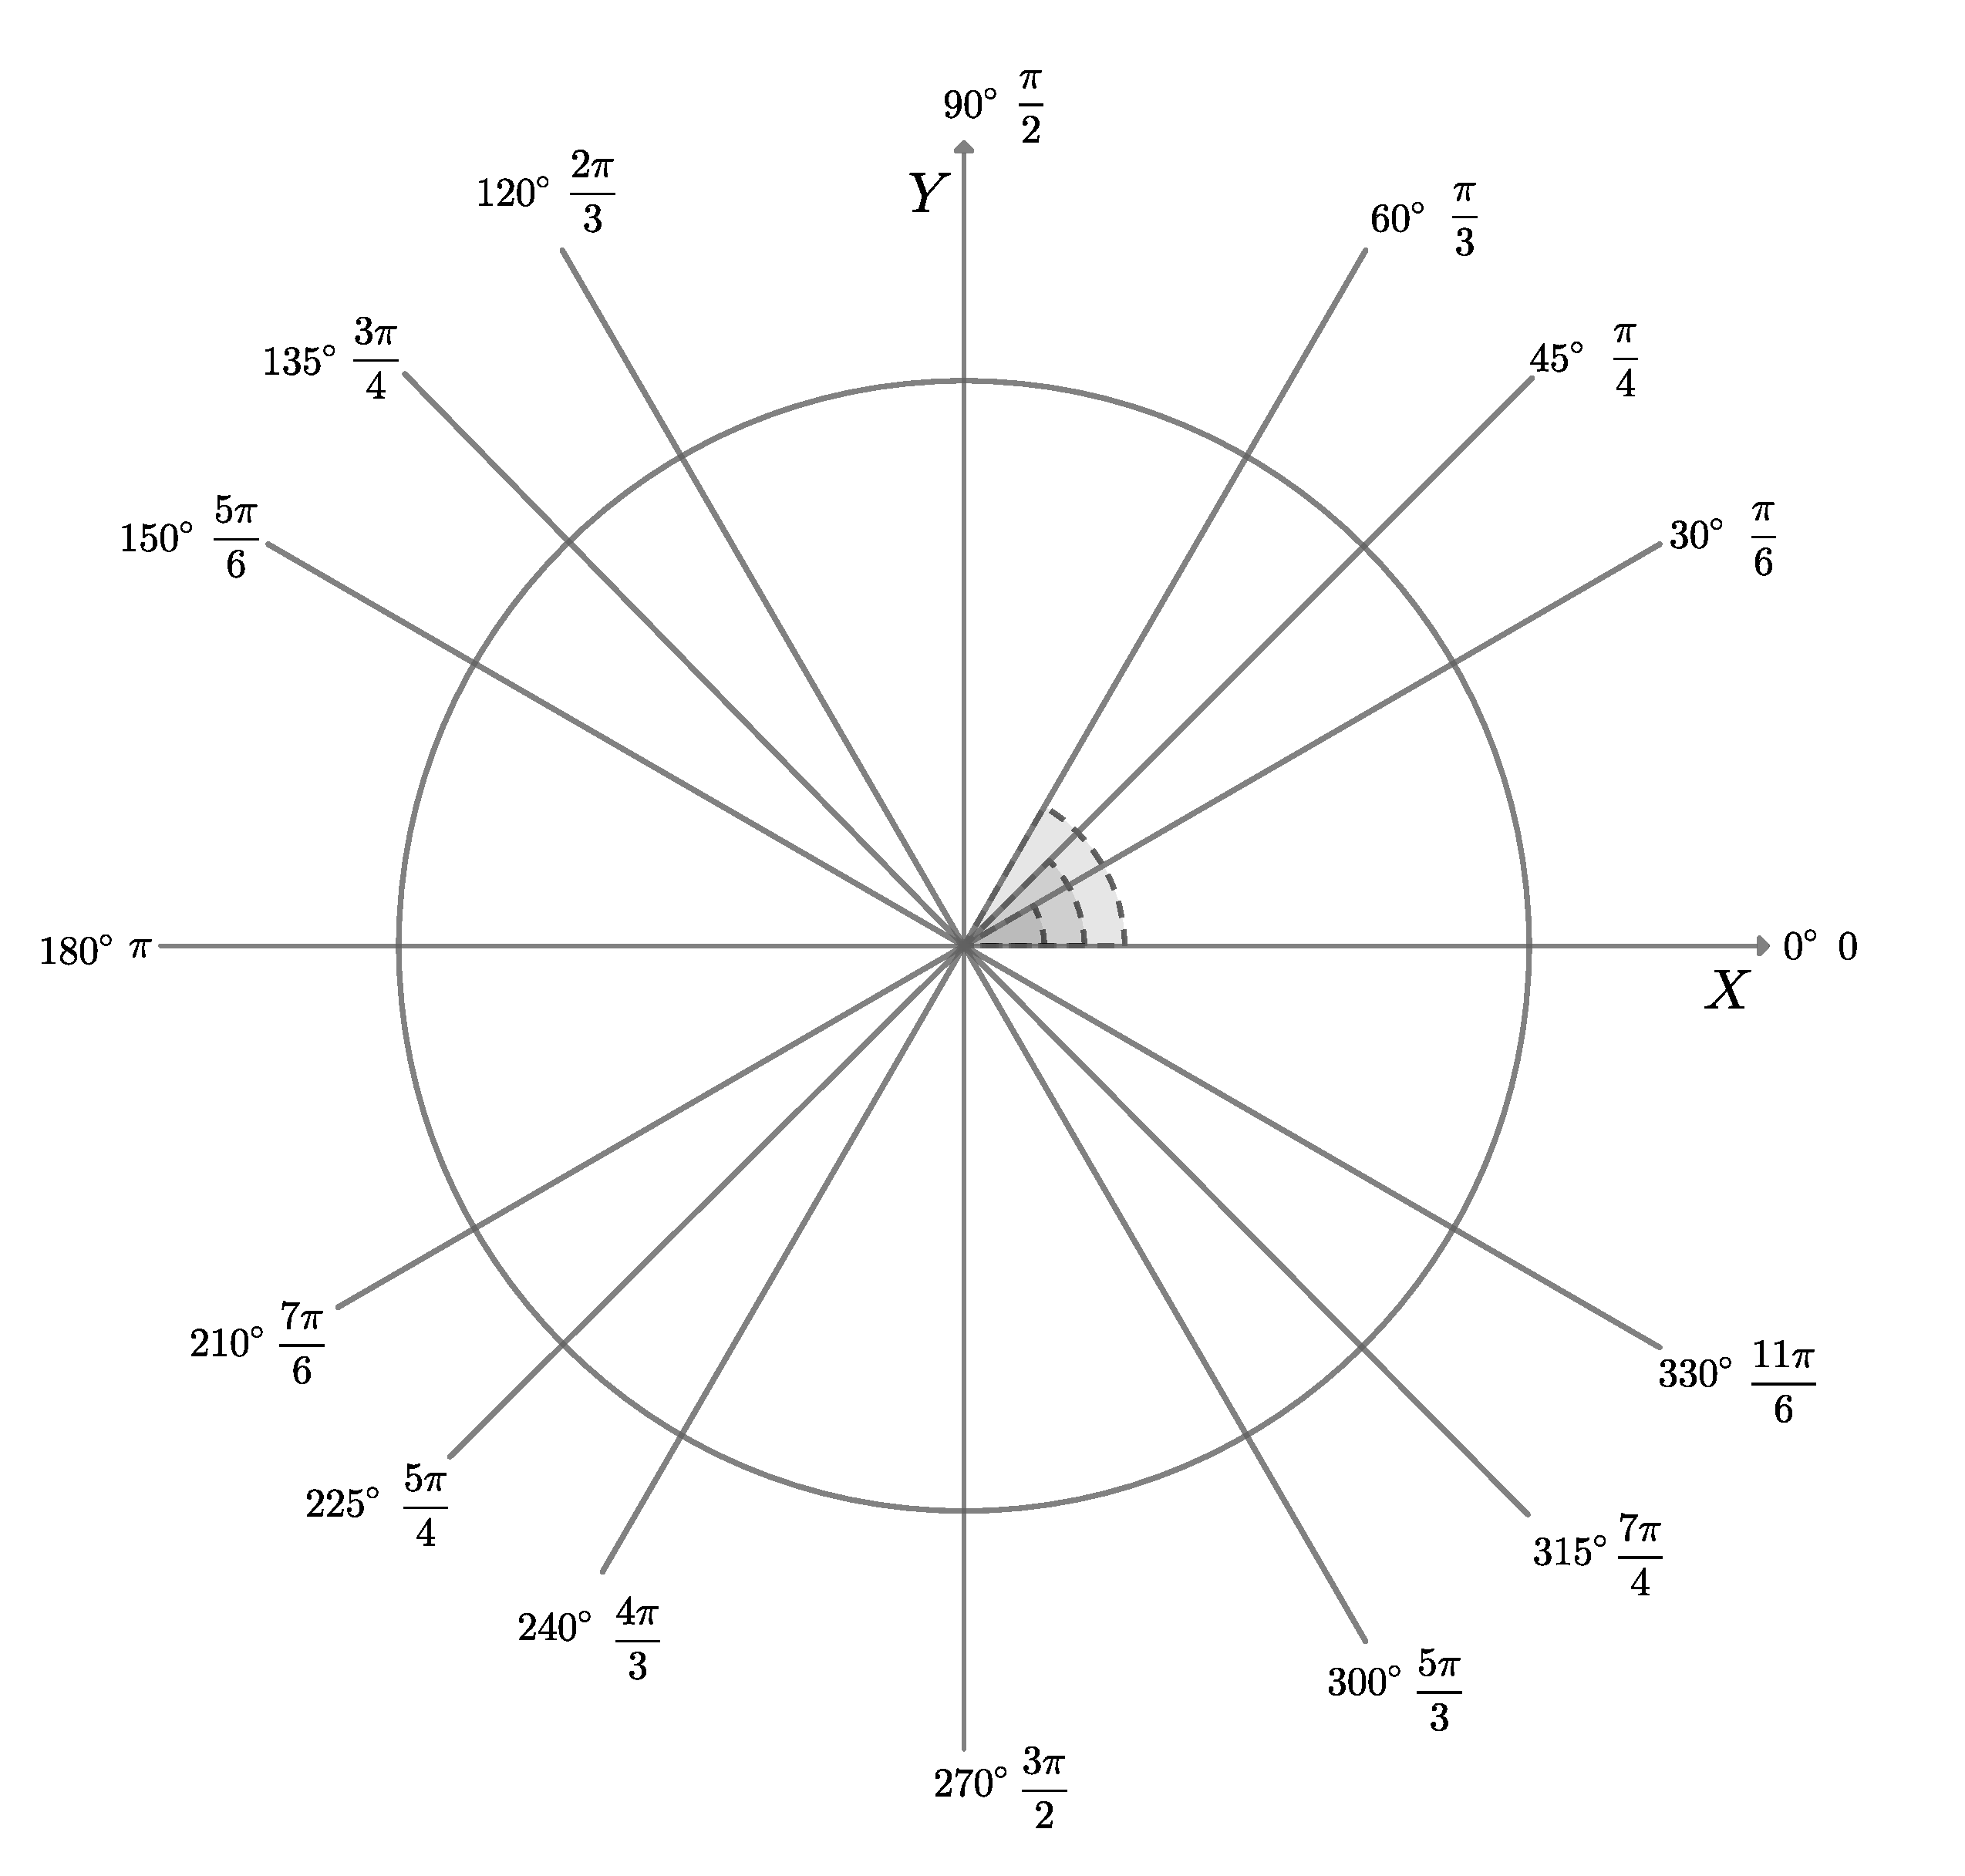
\includegraphics[scale=0.48]{51}
    	\caption{}
       \label{Figure51}
\end{figure} 
\newpage
\begin{examplebox}[NETSAT คณิตศาสตร์ สิงหาคม 2568]
กำหนดให้ $0<A<\dfrac{\pi}{2}$ และ $\tan(A)=2.4$ จงหาค่า $\cos(A)$
\begin{multicols}{2}
\begin{enumerate}
\item $\dfrac{5}{12}$
\item $\dfrac{5}{13}$
\item $-\dfrac{5}{12}$
\item $-\dfrac{5}{13}$
\end{enumerate}
\end{multicols}
\end{examplebox}
\newpage
\subsection{มุมคู่ $\pi$ และมุมคี่ $\pi$}
จากรูปที่~\ref{Figure53} สามารถจำแนกมุมที่เป็นพหุคูณของ $\pi$ ได้ดังนี้
\begin{itemize}
    \item \textbf{มุมคู่ $\pi$} คือ มุมที่สามารถเขียนได้ในรูป $2n\pi$ เมื่อ $n$ เป็นจำนวนเต็มไม่ลบ กล่าวคือ $n=0,1,2,\ldots$
    \item \textbf{มุมคี่ $\pi$} คือ มุมที่สามารถเขียนได้ในรูป $(2n+1)\pi$ เมื่อ $n$ เป็นจำนวนเต็มไม่ลบ กล่าวคือ $n=0,1,2,\ldots$
\end{itemize}
\begin{figure}[H]	 
	\centering
	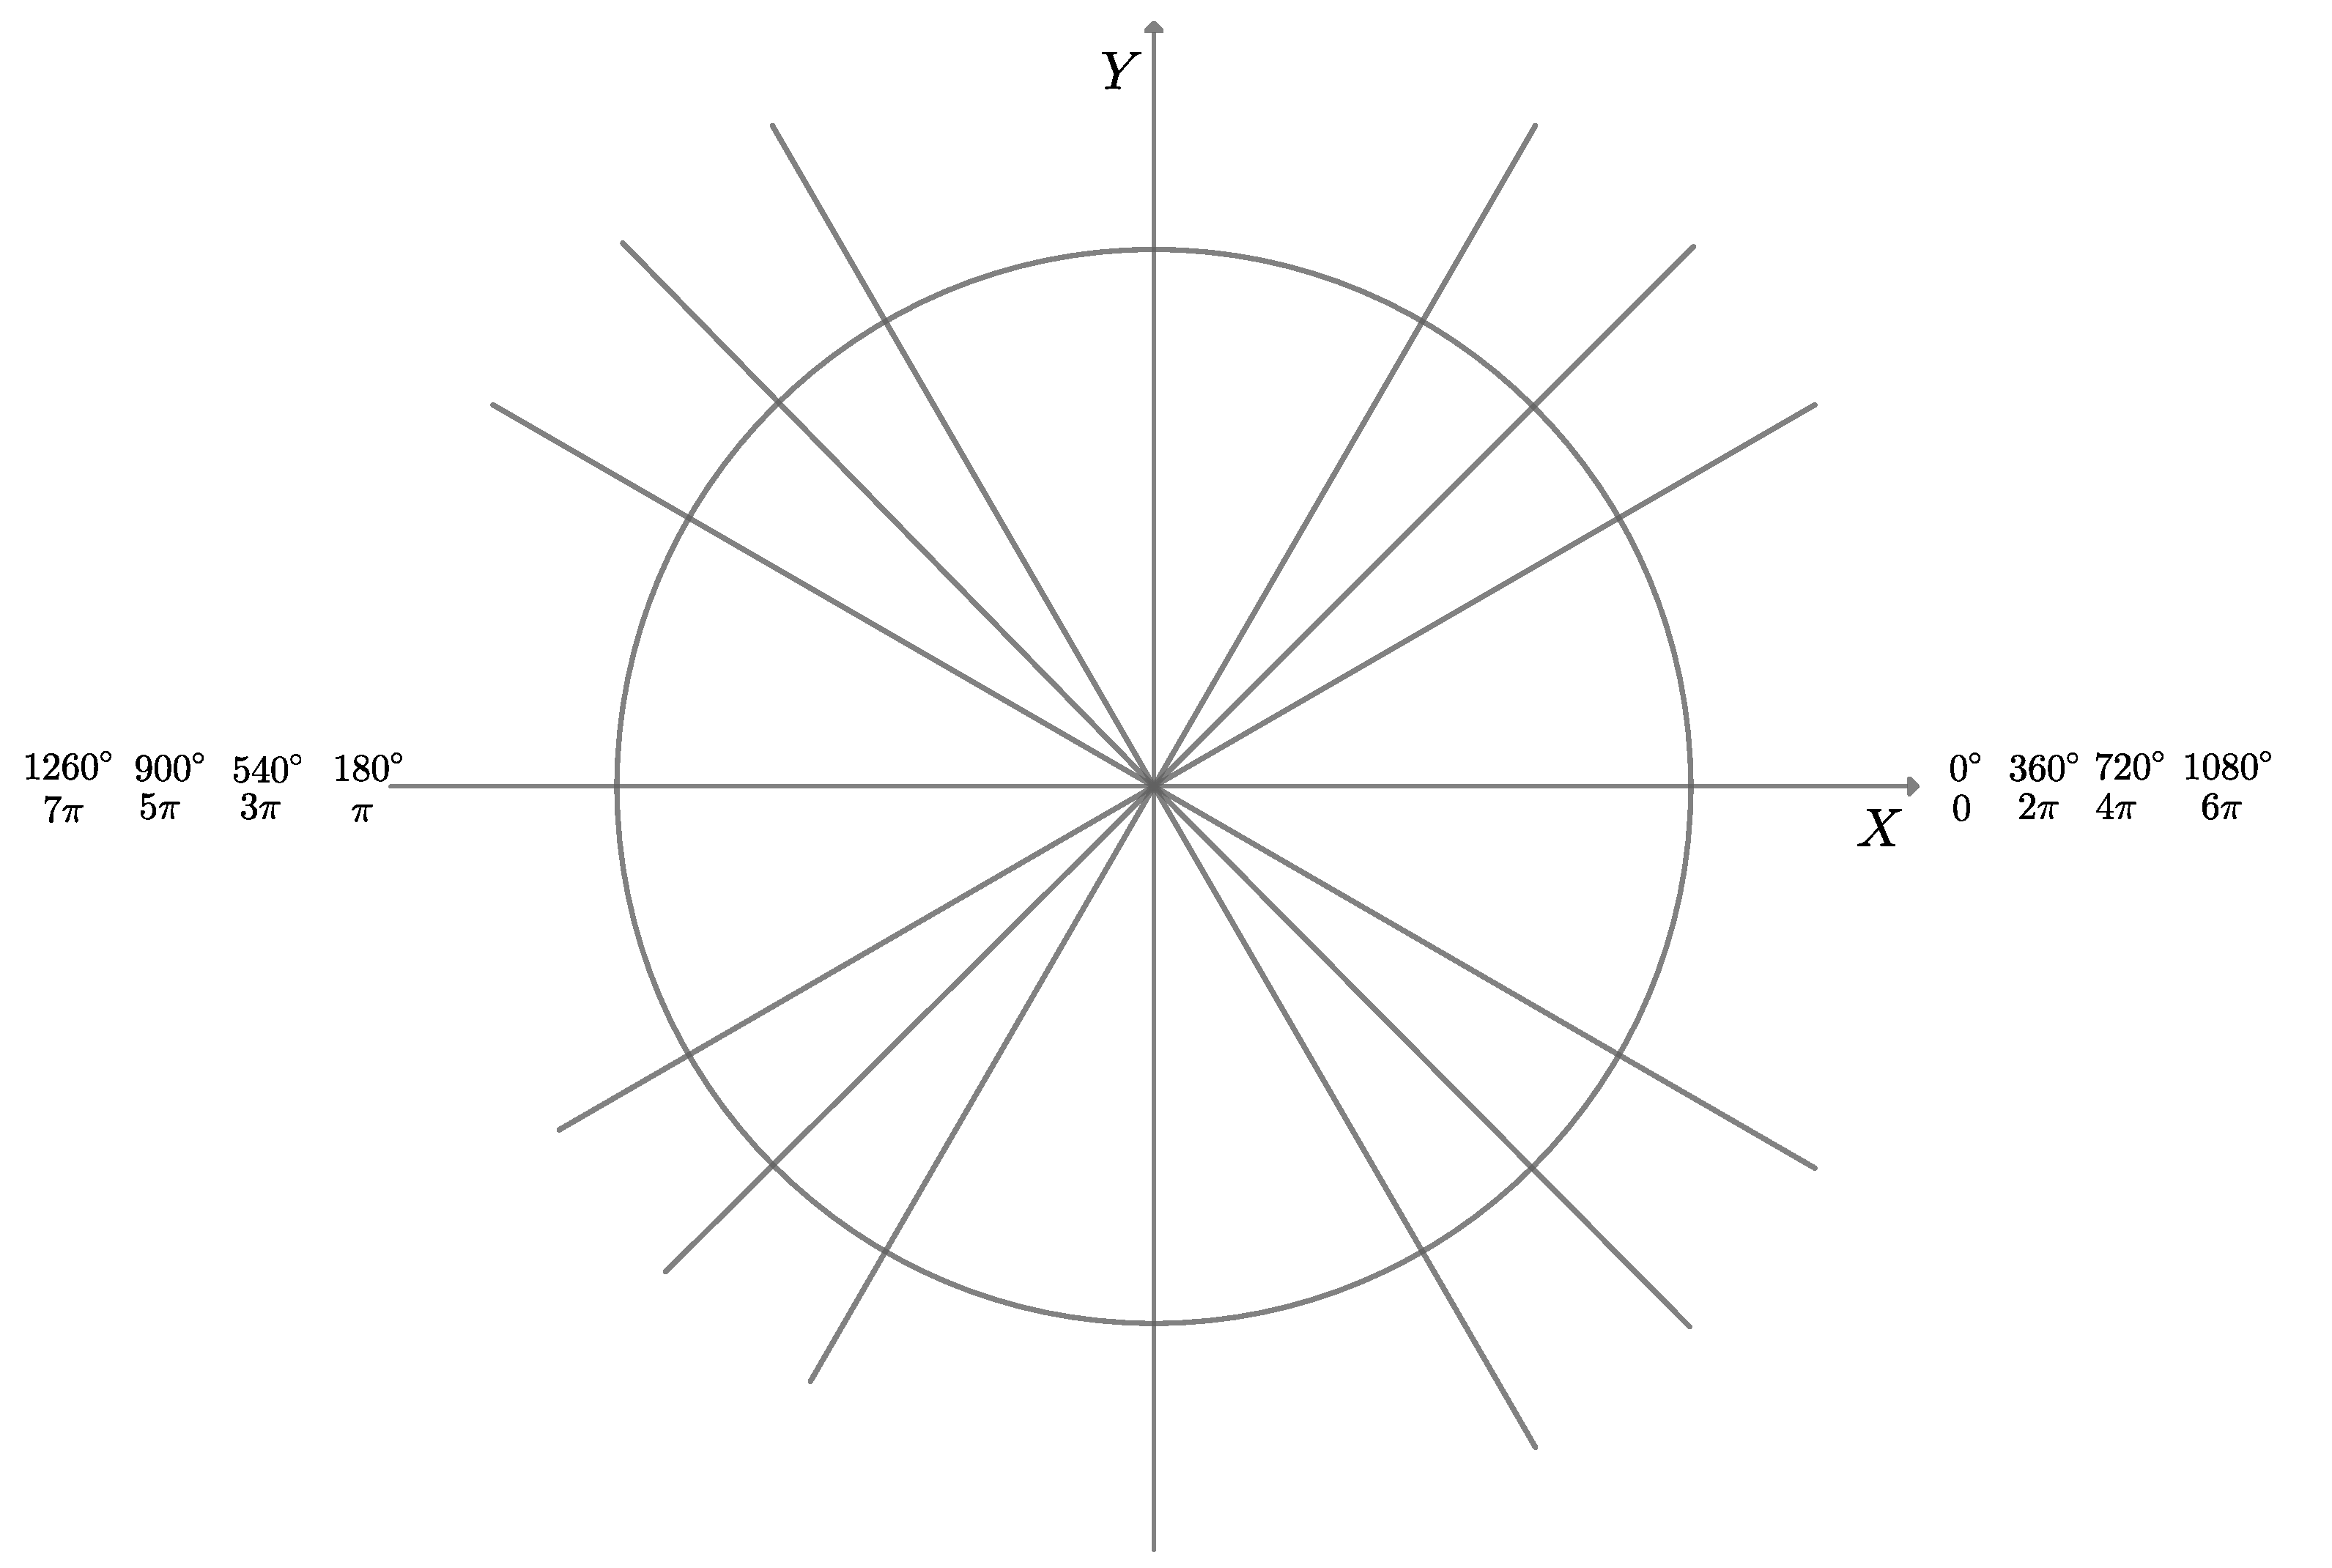
\includegraphics[scale=0.37]{53}
    	\caption{}
       \label{Figure53}
\end{figure} 

\newpage
\subsection{ค่าฟังก์ชันตรีโกณมิติของมุมเรเดียนในรูป $2n\pi \pm \theta$ และ $(2n+1)\pi \pm \theta$ 
เมื่อ $n$ เป็นจำนวนเต็มไม่ลบ}

\begin{conceptbox}\label{concept5.2}
ให้ $\alpha$ เป็นมุมในหน่วยเรเดียน สามารถหาค่าฟังก์ชันตรีโกณมิติของมุม $\alpha$ ได้ตามขั้นตอนดังนี้
\begin{enumerate}
    \item พิจารณาเครื่องหมายของมุม $\alpha$
    \begin{enumerate}[label*=\arabic*.]
        \item หาก $\alpha>0$ ให้ดำเนินการตามข้อ 2
        \item หาก $\alpha<0$ ให้ใช้สมบัติของฟังก์ชันตรีโกณมิติของมุมลบ 
        (ดูข้อควรรู้~\ref{remark1.3}) เพื่อแปลงเป็นมุมบวกก่อน แล้วจึงดำเนินการตามข้อ 2
    \end{enumerate}
    \item เขียนมุม $\alpha$ ให้อยู่ในรูป  
    \[
    2n\pi \pm \theta \quad \text{หรือ} \quad (2n+1)\pi \pm \theta
    \]
    เมื่อ $n$ เป็นจำนวนเต็มไม่ลบ และ $0<\theta<\dfrac{\pi}{2}$
    \item ตรวจสอบว่ามุมที่ได้อยู่ในควอดรันท์ใด
    \item ค่าฟังก์ชันตรีโกณมิติของมุม $\alpha$ จะเท่ากับ
    ค่าฟังก์ชันตรีโกณมิติของมุม $\theta$ 
    โดยพิจารณาเครื่องหมายของฟังก์ชันตามควอดรันท์นั้น
    (ตามที่กล่าวไว้ในหัวข้อย่อย~\ref{section1.4.1})
\end{enumerate}
\end{conceptbox}

\begin{examplebox}
จงหาค่าฟังก์ชันตรีโกณมิติต่อไปนี้ เมื่อกำหนดให้ $0<\theta<\dfrac{\pi}{2}$
\begin{enumerate}
    \item $\sin(3\pi+\theta)$  

    เนื่องจาก $3\pi+\theta$ อยู่ในควอดรันท์ที่ 3  
    \[
    \sin(3\pi+\theta)=-\sin(\theta)
    \]

    \item $\cos(2\pi+\theta)$  

    เนื่องจาก $2\pi+\theta$ อยู่ในควอดรันท์ที่ 1  
    \[
    \cos(2\pi+\theta)=\cos(\theta)
    \]

    \item $\tan(5\pi-\theta)$  

    เนื่องจาก $5\pi-\theta$ อยู่ในควอดรันท์ที่ 2  
    \[
    \tan(5\pi-\theta)=-\tan(\theta)
    \]
    
    \item $\cosec(10\pi-\theta)$  

    เนื่องจาก $10\pi-\theta$ อยู่ในควอดรันท์ที่ 4  
    \[
    \cosec(10\pi-\theta)=-\cosec(\theta)
    \]
\end{enumerate}
\end{examplebox}

\begin{examplebox}
จงหาค่าฟังก์ชันตรีโกณมิติต่อไปนี้ เมื่อกำหนดให้ $0<\theta<\dfrac{\pi}{2}$
\begin{enumerate}
    \item $\cot(\theta-\pi)$  
   \[
    \cot(\theta-\pi)
    =-\cot(\pi-\theta)
    \]
เนื่องจาก $\pi-\theta$ อยู่ในควอดรันท์ที่ 2 ดังนั้น $\cot(\pi-\theta)=-\cot(\theta)$\\
จึงได้ว่า
  \[
    \cot(\theta-\pi)
    =-(-\cot(\theta))
    =\cot(\theta)
    \]
    \item $\sec(-2\pi-\theta)$  
    \[
    \sec(-2\pi-\theta)
    =\sec(2\pi+\theta)
    \]
เนื่องจาก $2\pi+\theta$ อยู่ในควอดรันท์ที่ 1 ดังนั้น    
    \[
    \sec(-2\pi-\theta)
    =\sec(2\pi+\theta)
    =\sec(\theta)
    \]
\end{enumerate}
\end{examplebox}

\begin{examplebox}
จงหาค่าของ $\sin\left(\dfrac{8\pi}{3}\right)$
\end{examplebox}
\vspace{3cm}
\begin{examplebox}
จงหาค่าของ $\sin\left(-\dfrac{7\pi}{6}\right)$
\end{examplebox}
\vspace{3cm}
\begin{examplebox}
จงหาค่าของ $\cos\left(\dfrac{8\pi}{3}\right)$
\end{examplebox}
\vspace{3cm}
\begin{examplebox}
จงหาค่าของ $\cos\left(-\dfrac{11\pi}{3}\right)$
\end{examplebox}
\vspace{3cm}
\begin{examplebox}
จงหาค่าของ $\tan\left(\dfrac{4\pi}{3}\right)$
\end{examplebox}
\vspace{3cm}
\begin{examplebox}
จงหาค่าของ $\cosec\left(\dfrac{13\pi}{6}\right)$
\end{examplebox}
\vspace{3cm}
\begin{examplebox}
จงหาค่าของ $\tan\left(-\dfrac{13\pi}{6}\right)$
\end{examplebox}
\newpage
\begin{examplebox}
จงหาค่าของ $\cot\left(\dfrac{9\pi}{5}\right)$
\end{examplebox}
\vspace{3cm}
\begin{examplebox}
จงหาค่าของ 
\[\dfrac{\sin\left(\dfrac{3\pi}{8} \right)}{\sin\left(\dfrac{5\pi}{8} \right)}+ \dfrac{\tan\left(\dfrac{13\pi}{7}\right)}{\tan\left(\dfrac{\pi}{7} \right)}\]
\end{examplebox}
\newpage
\begin{observationbox}
จากหลักการ~\ref{concept5.2} เราสามารถประยุกต์ใช้เพื่อหาค่าฟังก์ชันตรีโกณมิติของมุมในหน่วยองศาได้ โดยมีแนวคิดเช่นเดียวกัน กล่าวคือ
ให้ $\alpha>0$ เป็นมุมในหน่วยองศา สามารถเขียนมุม $\alpha$ ให้อยู่ในรูป
\[
\left(n\times 180^{\circ}\right)\pm\theta
\]
เมื่อ $n$ เป็นจำนวนเต็มไม่ลบ กล่าวคือ $n=0,1,2,\ldots$ และ $0^{\circ}<\theta<90^{\circ}$
จากนั้นพิจารณาควอดรันท์ของมุมที่ได้ และกำหนดเครื่องหมายของฟังก์ชันตรีโกณมิติตามควอดรันท์นั้น โดยค่าฟังก์ชันตรีโกณมิติของมุม $\alpha$ จะเท่ากับค่าฟังก์ชันตรีโกณมิติของมุม $\theta$
\end{observationbox}


\begin{examplebox}
จงหาค่าของ $\cosec\left(150^{\circ}\right)$
\end{examplebox}
\vspace{3cm}
\begin{examplebox}
จงหาค่าของ $\sec\left(-315^{\circ}\right)$
\end{examplebox}
\vspace{3cm}
\begin{examplebox}
จงหาค่าของ $\cot\left(-1020^{\circ}\right)$
\end{examplebox}
\vspace{3cm}
\begin{examplebox}
จงหาค่าของ $\sin\left(210^{\circ}\right)$
\end{examplebox}
\newpage
\begin{examplebox}
จงหาค่าของ $\tan\left(-585^{\circ}\right)$
\end{examplebox}
\vspace{3cm}
\begin{examplebox}
จงหาค่าของ $\cos\left(765^{\circ}\right)$
\end{examplebox}
\vspace{3cm}
\begin{examplebox}
จงหาค่าของ 
\[\dfrac{\sin(-420^{\circ})\cot(210^{{\circ}})+\sqrt{3}\cot(-390^{{\circ}})-1}{\cos(-840^{\circ})}\]
\end{examplebox}
\newpage
\begin{examplebox}[NETSAT คณิตศาสตร์ สิงหาคม 2565]
ถ้า $A$ อยู่ในจตุภาคที่ 1 โดยที่ $0^{\circ}<A<90^{\circ}$ แล้ว $\cos(90^{\circ}-A)$ มีค่าเท่ากับเท่าใด
\begin{multicols}{2}
\begin{enumerate}
\item $\sin(A)$
\item $\cos(A)$
\item $-\sin(A)$
\item $-\cos(A)$
\end{enumerate}
\end{multicols}
\end{examplebox}
\newpage
\begin{examplebox}[NETSAT คณิตศาสตร์ สิงหาคม 2565]
กำหนด $0^{\circ}<A<90^{\circ}$ จงหาค่าของ 
\[\sin(90^{\circ}-A)\cos(A)\tan^2(A)+\dfrac{\sin(A) \cos(90^{\circ}-A)}{\tan^2(A)}\]
\begin{multicols}{2}
\begin{enumerate}
\item $-1$
\item $1$
\item $\sin(2A)$
\item $\cos(2A)$
\end{enumerate}
\end{multicols}
\end{examplebox}
\newpage
\begin{examplebox}[NETSAT คณิตศาสตร์ กุมภาพันธ์ 2565]
ถ้า $\tan(\theta)=-10$ เมื่อ $90^{\circ}<\theta<180^{\circ}$ แล้ว $\cos(\theta)$ มีค่าเท่าใด
\begin{multicols}{2}
\begin{enumerate}
\item $\dfrac{-1}{\sqrt{101}}$
\item $\dfrac{1}{\sqrt{101}}$
\item $\dfrac{10}{\sqrt{101}}$
\item $\dfrac{-10}{\sqrt{101}}$
\end{enumerate}
\end{multicols}
\end{examplebox}
\newpage
\begin{examplebox}[NETSAT คณิตศาสตร์ กุมภาพันธ์ 2565]
ถ้า $\theta$ เป็นมุม ซึ่ง $270^{\circ}<\theta<360^{\circ}$ และ $\sin(\theta)=-\dfrac{1}{4}$ แล้ว $\sin(2\theta)$ มีค่าเท่าใด
\begin{multicols}{2}
\begin{enumerate}
\item $-\dfrac{\sqrt{15}}{8}$
\item $\dfrac{\sqrt{15}}{8}$
\item $-\dfrac{\sqrt{15}}{4}$
\item $\dfrac{\sqrt{15}}{4}$
\end{enumerate}
\end{multicols}
\end{examplebox}

\newpage
\begin{examplebox}[NETSAT คณิตศาสตร์ สิงหาคม 2565]
ถ้า $\tan(\theta)=3$ สำหรับ $0^{\circ}<\theta<90^{\circ}$ แล้ว $\cos(\theta)+\sin( \theta)$ มีค่าเท่าใด
\begin{multicols}{2}
\begin{enumerate}
\item $\dfrac{1}{\sqrt{10}}$
\item $\dfrac{2}{\sqrt{10}}$
\item $\dfrac{3}{\sqrt{10}}$
\item $\dfrac{4}{\sqrt{10}}$
\end{enumerate}
\end{multicols}
\end{examplebox}
\newpage
\begin{examplebox}[NETSAT คณิตศาสตร์ สิงหาคม 2566]
ให้ $\theta=135^{\circ}$ และ $x=\cos(\theta), y=\sin(\theta)$ แล้ว $x-y$ มีค่าเท่าใด
\begin{multicols}{2}
\begin{enumerate}
\item $-\sqrt{2}$
\item $0$
\item $1$
\item $\sqrt{2}$
\end{enumerate}
\end{multicols}
\end{examplebox}
\newpage
\section{กฎของโคไซน์และกฎของไซน์}
\begin{theorembox}[กฎของโคไซน์]
กำหนดให้ $\triangle ABC$ เป็นสามเหลี่ยมใด ๆ
ซึ่งมีความยาวด้านตรงข้ามมุม $A,B$ และ $C$
เท่ากับ $a,b$ และ $c$ ตามลำดับ ดังรูปที่~\ref{Figure25}
จะได้ความสัมพันธ์ดังต่อไปนี้
\begin{align*}
a^2 &= b^2+c^2-2bc\cos(A)\\
b^2 &= c^2+a^2-2ca\cos(B)\\
c^2 &= a^2+b^2-2ab\cos(C)
\end{align*}
\end{theorembox}

\begin{figure}[H]
	\centering
	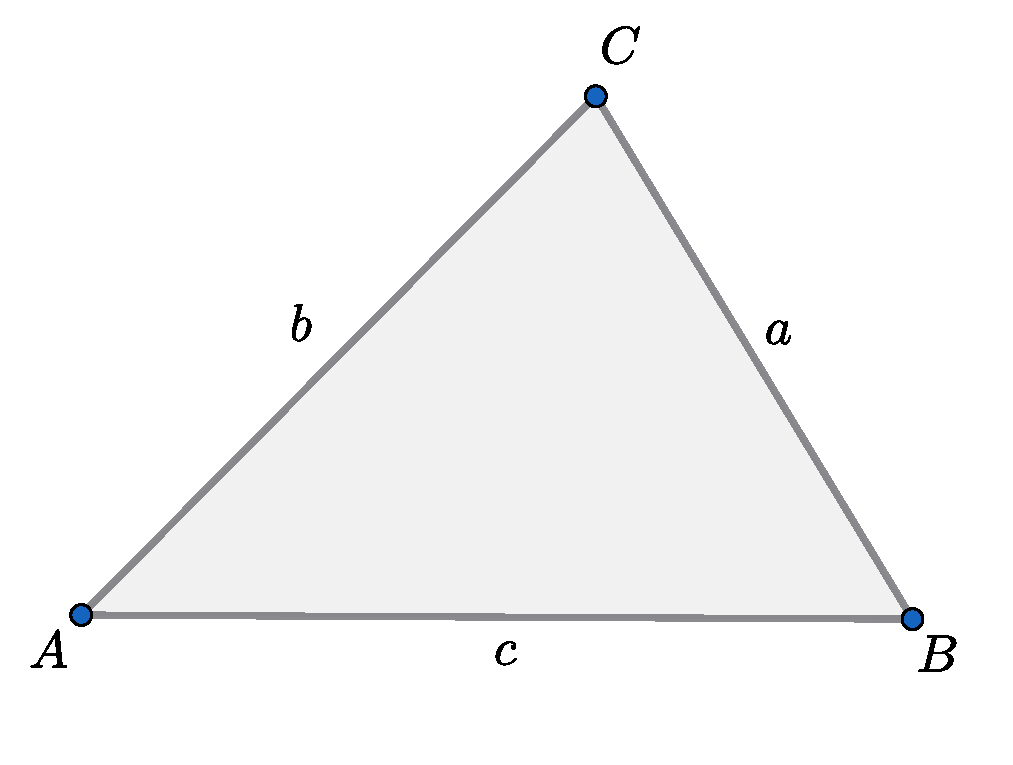
\includegraphics[scale=0.6]{25}
	\caption{}
	\label{Figure25}
\end{figure}

\newpage
\begin{theorembox}[กฎของไซน์]
กำหนดให้ $\triangle ABC$ เป็นสามเหลี่ยมใด ๆ
ซึ่งถูกล้อมรอบด้วยวงกลมรัศมี $R$
และมีความยาวด้านตรงข้ามมุม $A,B$ และ $C$
เท่ากับ $a,b$ และ $c$ ตามลำดับ ดังรูปที่~\ref{Figure26}
จะได้ความสัมพันธ์ว่า
\[
\frac{a}{\sin(A)}=\frac{b}{\sin(B)}=\frac{c}{\sin(C)}=2R
\]
\end{theorembox}

\begin{figure}[H]
	\centering
	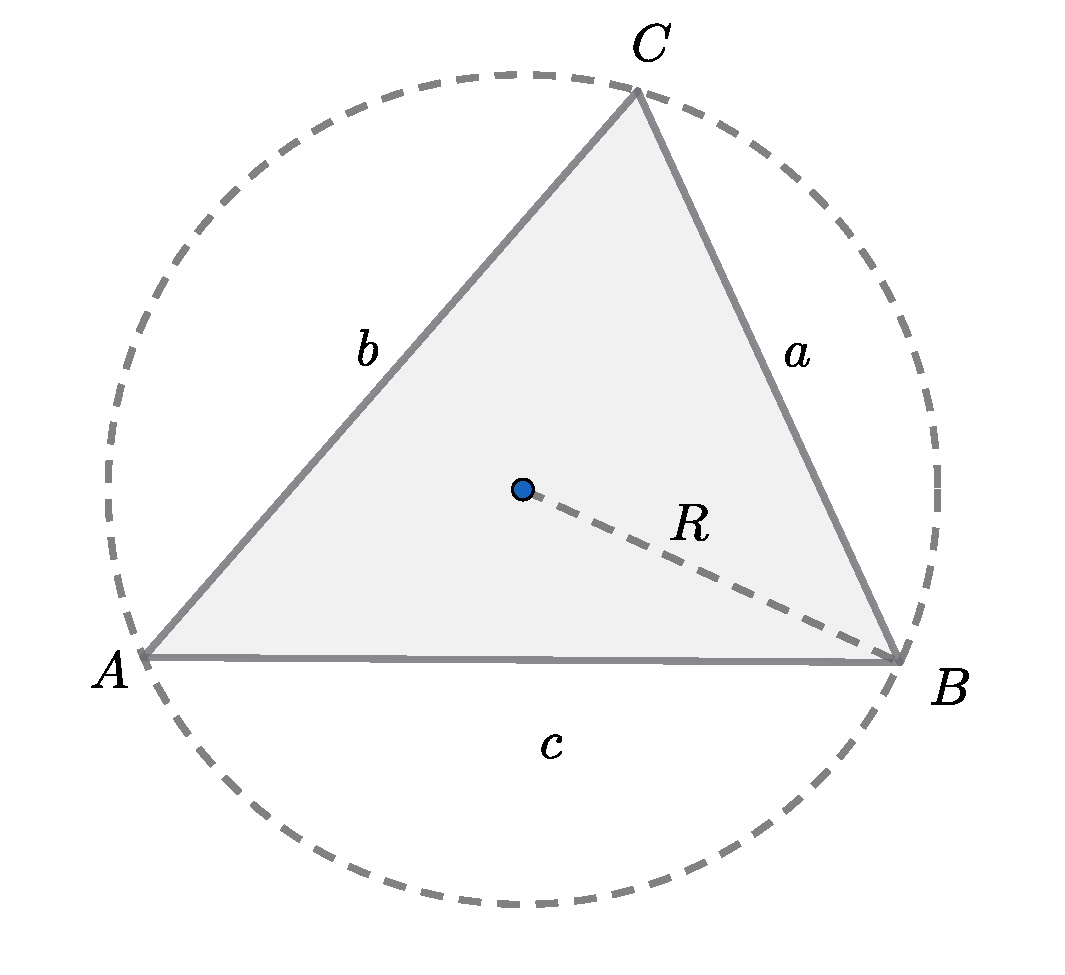
\includegraphics[scale=0.5]{26}
	\caption{}
	\label{Figure26}
\end{figure}

\begin{examplebox}[NETSAT คณิตศาสตร์ สิงหาคม 2568]  
กำหนดให้ $\triangle ABC$ มี $AB=3$ หน่วย $AC=3$ หน่วย และ $\angle A =120^{\circ}$ จงหาความยาวด้าน $BC$
\begin{multicols}{2}
\begin{enumerate}
\item $3\sqrt{3}$
\item $3\sqrt{5}$
\item $3\sqrt{7}$
\item $9$
\end{enumerate}
\end{multicols}
\end{examplebox}
\newpage
\begin{examplebox}[NETSAT คณิตศาสตร์ กุมภาพันธ์ 2565]
กำหนดให้ $\triangle A B C$ มีความยาวด้าน $BC$ คือ $a$ หน่วย มีความยาวด้าน $CA$ คือ $b$ หน่วย มีความยาวด้าน $AB$ คือ $c$ หน่วย และยังสอดคล้องกับเงื่อนไข
\[3(a+b)(a-b)=c(2 b+3 c)\]
แล้ว $\tan(A)$ มีค่าเท่าใด
\begin{multicols}{2}
\begin{enumerate}
\item $\dfrac{1}{2 \sqrt{2}}$
\item $-\dfrac{1}{2 \sqrt{2}}$
\item $2 \sqrt{2}$
\item $-2 \sqrt{2}$
\end{enumerate}
\end{multicols}
\end{examplebox}
\newpage
\begin{examplebox}[NETSAT คณิตศาสตร์ กุมภาพันธ์ 2565]
ให้ $\alpha$ และ $\beta$ เป็นค่าคงตัว ซึ่ง $0<\alpha<\beta<2\pi$ \\
กำหนดให้ฟังก์ชัน
\[f(x)=\sin^2(x)+\sin^2(x+\beta)+\sin^2(x+\beta)\,\, \text{มีค่าเป็นค่าคงตัว $c$ สำหรับ $0 \leq x \leq 2 \pi$}\]
แล้ว $c$ มีค่าเท่าไร
\begin{multicols}{2}
\begin{enumerate}
\item $0$
\item $1$
\item $\dfrac{3}{2}$
\item $2$
\end{enumerate}
\end{multicols}
\end{examplebox}
\newpage
\begin{examplebox}[NETSAT คณิตศาสตร์ 2566]
จากรูปที่~\ref{Figure27} จงหาขนาดของมุม $B$
\begin{multicols}{2}
\begin{enumerate}
\item $30^{\circ}$
\item $45^{\circ}$
\item $60^{\circ}$
\item $75^{\circ}$
\end{enumerate}
\end{multicols}
\end{examplebox} 
\begin{figure}[H]	 
	\centering
	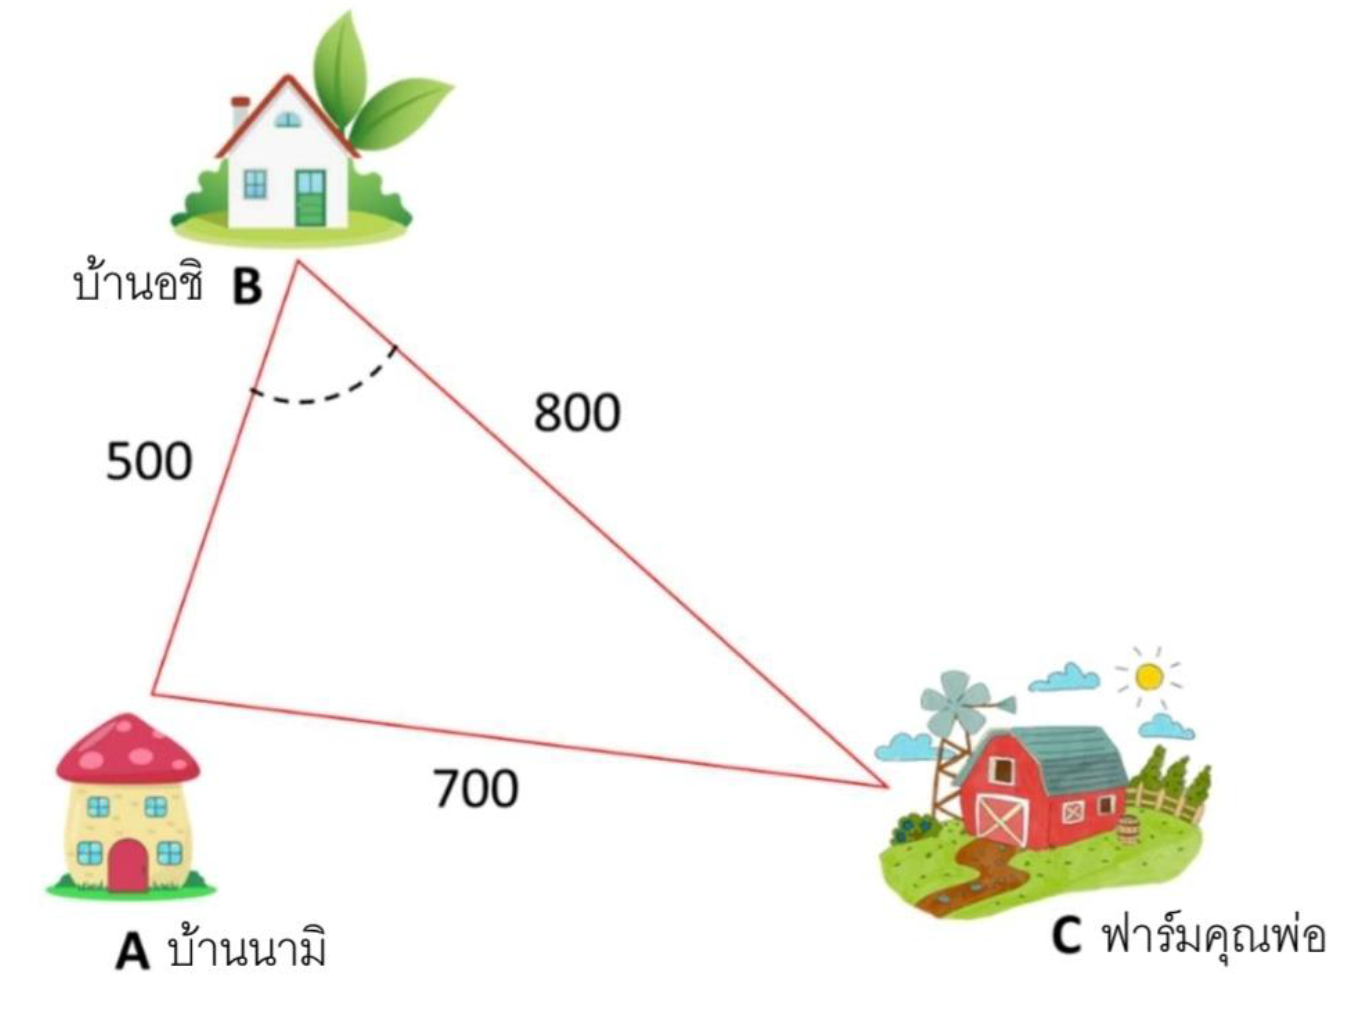
\includegraphics[scale=0.5]{27}
    	\caption{}
       \label{Figure27}
\end{figure} 
\newpage
\begin{examplebox}[NETSAT คณิตศาสตร์ 2566]
จากรูปที่~\ref{Figure27} นามิและอชินัดพบกันที่จุด $O$ ซึ่งอยู่ห่างจากบ้านของนามิ บ้านของอชิ และฟาร์มคุณพ่อ เป็นระยะเท่ากัน จงหาระยะทางโดยประมาณจากบ้านของบ้านของอชิและฟาร์มคุณพ่อไปยังจุด $O$ ที่ใกล้เคียงมากที่สุด โดยกำหนดให้ $\sqrt{3}=1.73$
\begin{multicols}{2}
\begin{enumerate}
\item $300$ เมตร
\item $400$ เมตร
\item $500$ เมตร
\item $600$ เมตร
\end{enumerate}
\end{multicols}
\end{examplebox} 
\newpage
\begin{examplebox}[NETSAT คณิตศาสตร์ 2566]
รูปที่~\ref{Figure28} แสดงภาพมุมสูงของม้าหมุนในสวนแห่งหนึ่ง โดยมีที่นั่งอยู่บนเส้นรอบวงสองวงและหมุนรอบจุดศูนย์กลาง $O$ โดยมีรัศมีของวงกลมด้านนอกเท่ากับ $10$ เมตร รัศมีของวงกลมด้านในเท่ากับ $6$ เมตร
กำหนดให้ที่นั่ง $A$ และ $B$ อยู่ข้างกันบนเส้นรอบวงด้านนอกและด้านในตามลำดับโดยไม่คำนึงขนาดของที่นั่ง เมื่อที่นั่ง $A$ และ $B$ เริ่มขยับไปพร้อมๆ กัน รูปที่ 2 แสดงให้เห็นตำแหน่ง $A$ และ $B$ หลังผ่านไป $2-3$ นาที หลังจากเริ่มหมุน ถ้า $\angle AOB=\theta$ และ $\cos(\theta)=\dfrac{11}{24}$ จงหาระยะทางจาก $A$ มา $B$
\begin{multicols}{2}
\begin{enumerate}
\item $7$
\item $9$
\item $11$
\item $13$
\end{enumerate}
\end{multicols}
\end{examplebox} 
\begin{figure}[H]	 
	\centering
	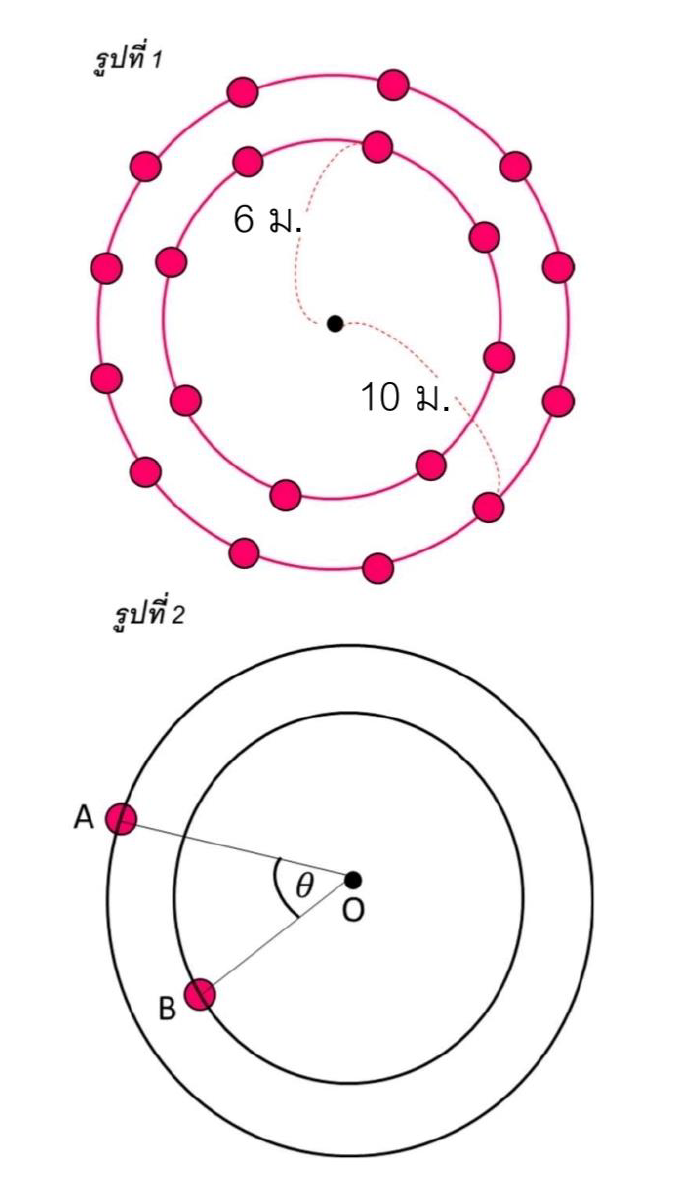
\includegraphics[scale=0.7]{28}
    	\caption{}
       \label{Figure28}
\end{figure}

\newpage
\thispagestyle{empty}
\begin{remarkbox}
วงกลมวงหนึ่งและวงเดียวเท่ากันที่สามารถผ่านจุดทั้งสามจุดที่ไม่อยู่ในแนวเส้นตรงเดียวกัน\\
จากรูปที่~\ref{Figure62} กำหนดให้จุด $A,B$ และ $C$ เป็นจุดสามจุดที่ไม่อยู่ในแนวเส้นตรงเดียวกัน จึงสามารถถูกวงกลมเพียงวงเดียวผ่านทั้งสามจุด
\end{remarkbox}

\begin{figure}[H]
	\centering
	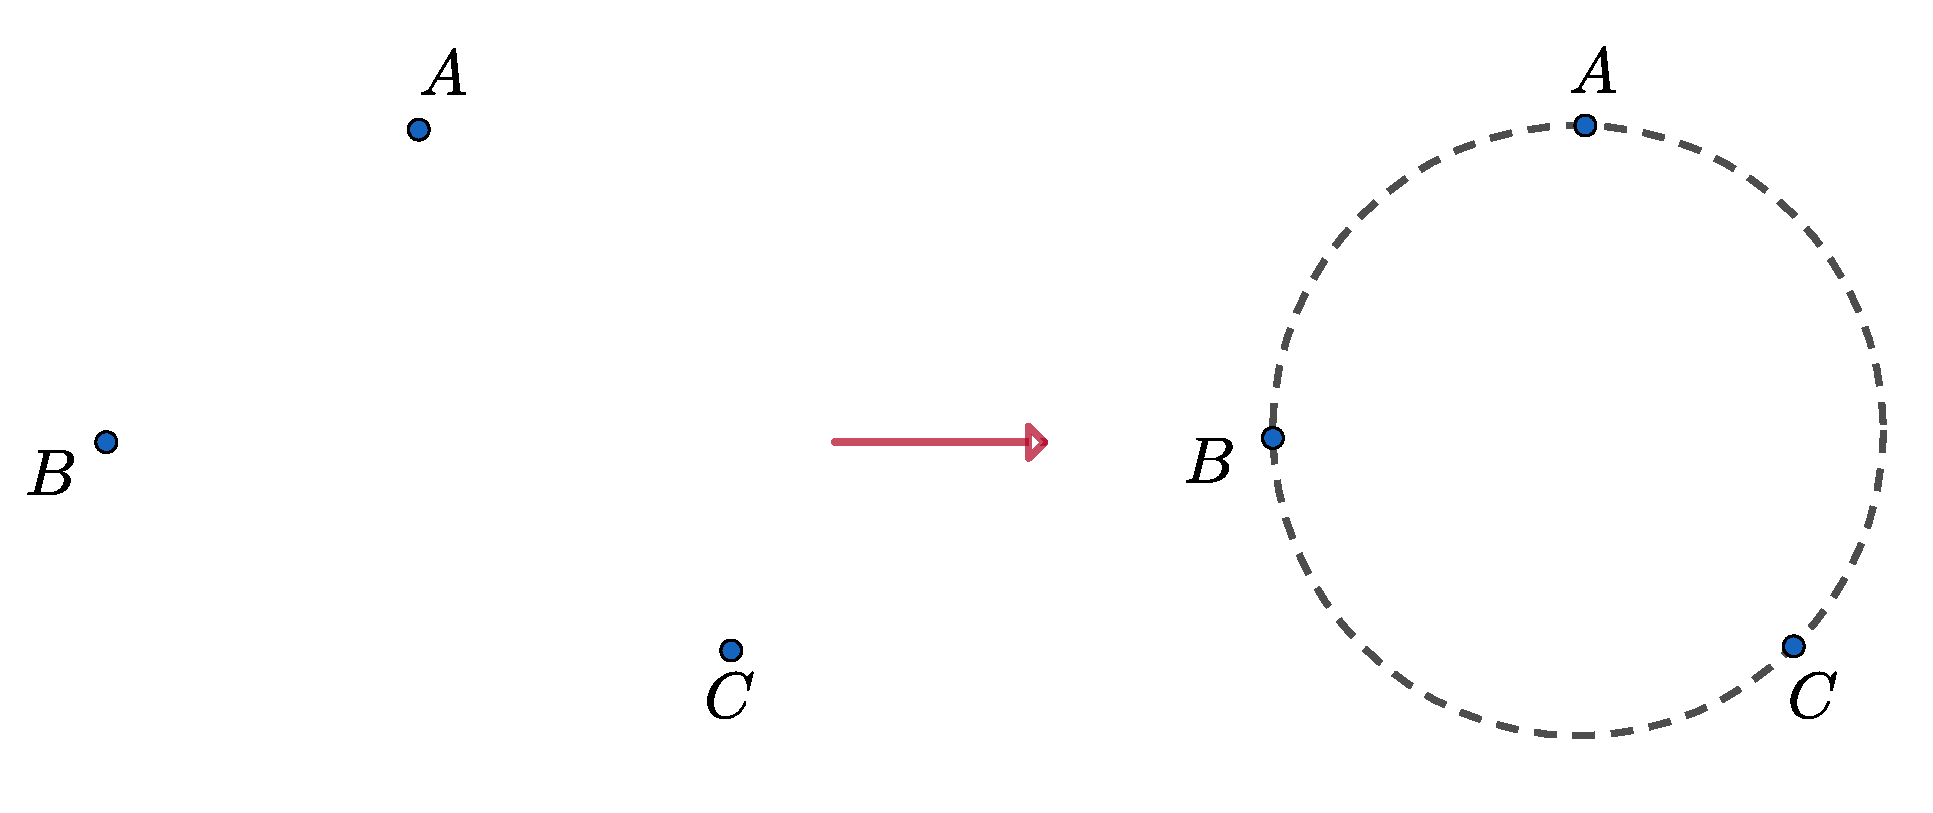
\includegraphics[scale=0.55]{62}
	\caption{}
	\label{Figure62}
\end{figure}

\begin{remarkbox}
จากจุดจุดหนึ่งภายในวงกลม ถ้าลากส่วนของเส้นตรงไปยังเส้นรอบวงให้ยาวเท่ากันได้ \textbf{มากกว่าสองเส้นขึ้นไป} แล้วจุดนั้นจะเป็นจุดศูนย์กลางของวงกลม\\
จากรูปที่~\ref{Figure63} ลากส่วนของเส้นตรงจากจุด $O$ ไปยังจุด $A,B$ และ $C$ ที่อยู่บนเส้นรอบวงได้ความยาวเท่ากัน จึงสามารถสรุปได้ว่าจุด $O$ เป็นจุดศูนย์กลางของวงกลม
\end{remarkbox}
\begin{figure}[H]
	\centering
	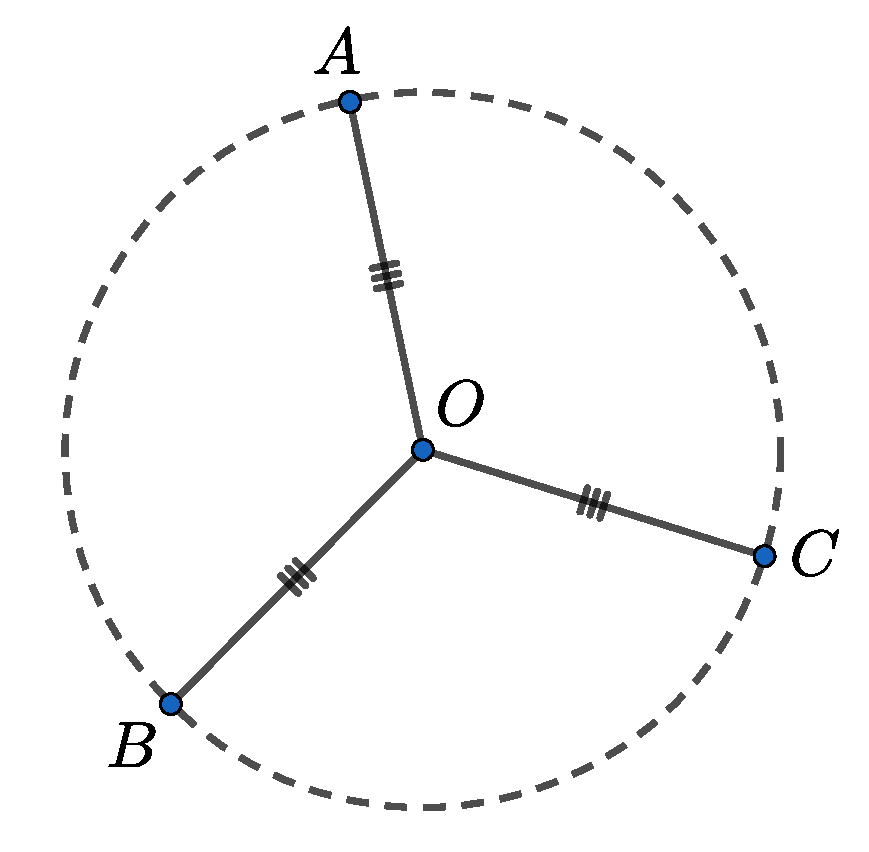
\includegraphics[scale=0.52]{63}
	\caption{}
	\label{Figure63}
\end{figure}

		
\end{document}